\begin{document}

\classname{Algebra: Chapter 0, Paolo Aluffi}
\typeofarticle{Exercises solutions}

\maketitle

\tableofcontents

\everymath{\dis}

\newpage
\begin{center}
\fbox{
\parbox{13cm}{
Copyright (C) 2023 doyoung @ \href{https://github.com/choco-bear/}{https://github.com/choco-bear/}. \\
Permission is granted to copy, distribute and/or modify this
document under the terms of the GNU Free Documentation License,
Version 3.0 or any later version published by the Free Software
Foundation; with the Invariant Sections being just "GNU
Manifesto" and just "Prologue", with no Front-Cover Texts, and with no Back-Cover
Texts.  A copy of the license is included in the section
entitled "GNU Free Documentation License".
}}

%\vspace{48pt}
%\emph{Special thanks to the following contributers:}
\end{center}

\chapter*{Prologue}
\addcontentsline{toc}{chapter}{Prologue}

\section*{Introduction}
\addcontentsline{toc}{section}{Introduction}
\markboth{\MakeUppercase{Prologue}}{\MakeUppercase{Introduction}}

``Algebra: Chapter 0." Even the title of this textbook suggests a beginning, a starting point, a foundation from which to explore the complex and captivating world of algebra. It's a signal to the reader that this is where the journey begins, an invitation to set out on a path filled with intriguing problems, elegant solutions, and a deeper understanding of the mathematical principles that govern our world.

As an undergraduate student, I found myself drawn to this beginning, to ``Chapter 0," and to the idea of delving into algebra from the ground up. My curiosity was piqued, but I also recognized that curiosity alone might not be enough to navigate the intricacies of algebra. The challenges could be overwhelming, the concepts elusive, and the solutions often just out of reach.

That realization led me to embark on a personal journey of self-study and exploration, and this solution manual is the result.

In these pages, I have documented my path through ``Algebra: Chapter 0," providing solutions, insights, and explanations along the way. This manual is not the work of an expert; it's the work of a fellow traveler, one who has grappled with the same questions, puzzled over the same problems, and rejoiced in the same moments of understanding.

My goal is to make this journey more accessible to others who are drawn to the world of algebra. Whether you're a fellow student, a teacher, or simply someone with a curiosity about mathematics, I hope you'll find value in these pages. Each solution is presented with clarity and care, reflecting not only the method to arrive at the answer but the thought process and insights that led me there.

So, here's to ``Chapter 0," to beginnings, and to the joy of learning. Join me on this adventure, and let's explore the fascinating landscape of algebra together. Let's embrace the challenges, celebrate the discoveries, and take pleasure in the knowledge that we are part of a community of learners, all striving to understand, all starting from the same point: Chapter 0.

Welcome to the journey.

\newpage
\section*{Some important points}
\addcontentsline{toc}{section}{Some important points}
\markboth{\MakeUppercase{Prologue}}{\MakeUppercase{Some important points}}
There are a few important points to note here:
\begin{itemize}
    \item The solution is \emph{only} hosted on my GitHub page
        \begin{center}
		  \href{https://github.com/choco-bear/algebra-chapter-0-solutions}{https://github.com/choco-bear/algebra-chapter-0-solutions}.
        \end{center} 
        If you find this document outside this page, you might have an outdated version of the solution which might have errors, so please be aware.
    \item I will update the solution irregularly.
    \item I've tried to reflect errata \href{https://www.math.fsu.edu/~aluffi/algebraerrata.2009/Errata.html}{https://www.math.fsu.edu/~aluffi/algebraerrata.2009/Errata.html} as much as possible.
    \item If you found an error in the solutions, typos, bad grammar or want to give an advise on LaTeX formatting, etc., don't hesitate to open an issue or a pull request on my repo. 
\end{itemize}

Best,

\begin{flushright}
doyoung @ \href{https://github.com/choco-bear/}{https://github.com/choco-bear/} \\
Department of Computer Science \& Engineering, Seoul National University \\
Updated \specialdate\today \\
v1.5.12
\end{flushright}
\chapter{Preliminaries: Set theory and categories}
\section{Naive set theory}
\problem{
    Locate a discussion of Russell's paradox, and understand it.
}{
    Recall that, in naive set theory, any collection of objects satisfying some properties can be called a set. Russel's paradox can be illustrated as follows:

    Let $R$ be the set of all sets that do not contain themselves. Then, if $R \notin R$, then by definition it must be the case that $R \in R$. Similarly, if $R \in R$ then it must be the case that $R \notin R$.

    This is the reason why we need the axiomatic set theory instead of the naive set theory.
}

\problem{
    $\vartriangleright$ Prove that if $\sim$ is an equivalence relation on a set $S$, then the corresponding family $\mathscr{P}_\sim$ defined in \S 1.5 is indeed a partition of $S$; that is, its elements are nonempty, disjoint, and their union is $S$. $\left[ \text{\S1.5} \right]$
}{
    Let $S$ be a set with an equivalence relation $\sim$. Consider the family of equivalence classes with respect to $\sim$ over $S$:
    $$\mathscr{P}_\sim = \{ \left[ a \right]_\sim \mid a \in S \}$$

    Let $\left[ a \right]_\sim \in \mathscr{P}_\sim$. Then by reflexivity of $\sim$, we have $a \sim a$ and thus $\left[ a \right]_\sim$ is nonempty. 

    Now, take any two elements $\left[ a \right]_\sim$ and $\left[ b \right]_\sim$ of $\mathscr{P}_\sim$. If $\left[ a \right]_\sim \cap \left[ b \right]_\sim$ is nonempty, then we can take an element $c \in \left[ a \right]_\sim \cap \left[ b \right]_\sim$. By definition, we get $c \sim a$ and $c \sim b$. By symmetricity of $\sim$, we get $a \sim c$ and so $a \sim b$ by transitivity of $\sim$. This means that $a \in \left[ b \right]_\sim$, and by transitivity of $\sim$, we can conclude that $\left[ a \right]_\sim \subseteq \left[ b \right]_\sim$.

    In the same way, we also can conclude that $\left[ b \right]_\sim \subseteq \left[ a \right]_\sim$ when $\left[ a \right]_\sim \cap \left[ b \right]_\sim$ is nonempty, and hence $\left[ a \right]_\sim = \left[ b \right]_\sim$ if $\left[ a \right]_\sim \cap \left[ b \right]_\sim$ is nonempty. In the other words, the elements of $\mathscr{P}_\sim$ are disjoint.
    
    Finally, for any $a \in S$, $a \in \left[ a \right]_\sim$, and thus $S \subseteq \bigcup \mathscr{P}_\sim$, obviously. Also, since $\sim$ is a relation on the set $S$, $\bigcup \mathscr{P}_\sim \subseteq S$, indeed.

    Therefore, $\mathscr{P}_\sim$ is a partition of $S$.
}

\problem{
    $\vartriangleright$ Given a partition $\mathscr{P}$ on a set $S$, show how to define an equivalence relation $\sim$ on $S$ such that $\mathscr{P}$ is the corresponding partition. $\left[ \text{\S1.5} \right]$
}{
    Let $S$ be a set with a partition $\mathscr{P}$. Consider a relation $\sim$ on $S$ as:
    $$a \sim b \iff \exists P \in \mathscr{P} \st a,b \in P.$$

    Then, it is quite obvious that $\sim$ is an equivalence relation.
}

\problem{
    How many different equivalence relations may be defined on the set $\{ 1,2,3 \}$?
}{
    Since there is a correspondence between equivalence relations and partitions, the number of equivalence relations is the same with the number of partitions. Since there are 5 different partitions of the set $\{ 1,2,3 \}$, there are 5 different equivalence relations can be defined on the set $\{ 1,2,3 \}$.
}

\problem{
    Give an example of a relation that is reflexive and symmetric but not transitive. What happens if you attempt to use this relation to define a partition on the set?
}{
    For $a,b \in \RR$, define $a \mathrel{\mathcal{R}} b$ to be true if and only if $\abs{a-b} \leq 1$. Then, it is obvious that $\mathrel{\mathcal{R}}$ is reflexive and symmetric. However, since $0 \not\mathrel{\mathcal{R}} 2$ even though $0 \mathrel{\mathcal{R}} 1$ and $1 \mathrel{\mathcal{R}} 2$, $\mathrel{\mathcal{R}}$ is not transitive. The corresponding family $\mathscr{P}_{\mathrel{\mathcal{R}}}$, defined as in \S 1.5, is not a partition of $\RR$, indeed  because the elements of $\mathscr{P}_{\mathrel{\mathcal{R}}}$ are not disjoint.
}

\problem{
    $\vartriangleright$ Define a relation $\sim$ on the set $\RR$ of real numbers by setting $a \sim b \iff b-a \in \ZZ$.  Prove that this is an equivalence relation, and find a `compelling' description for $\RR / \sim$. Do the same for the relation $\approx$ on the plane $\RR \times \RR$ defined by declaring  $\left( a_1,a_2 \right) \approx \left( b_1,b_2 \right) \iff b_1 - a_1 \in \ZZ$ and $b_2 - a_2 \in \ZZ$.  $\left[ \text{\S{}II.8.1, II.8.10} \right]$
}{
    Since $0 \in \ZZ$, $-n \in \ZZ$ for any $n \in \ZZ$, and $n+m \in \ZZ$ for any $n,m \in \ZZ$, the given relation $\sim$ on $\RR$ is an equivalence relation. Moreover, $\RR / \sim$ can be considered as $\lcint{0}{1}$ with operation on modulo 1. (It can be considered as $S^1$.)

    Now define a relation $\approx$ on $\RR^2$ by setting $\left( a_1,a_2 \right) \approx \left( b_1,b_2 \right) \iff a_1 - a_2 \in \ZZ$ and $b_1 - b_2 \in \ZZ$. Then by the similar way with the above, the relation $\approx$ on $\RR^2$ is an equivalence relation. Additionally, $\RR^2 / \approx$ is isomorphic to $\lcint{0}{1} \times \lcint{0}{1}$ with operation on modulo 1. (It can be considered as $T^2$.)
}

\newpage
\section{Functions between Sets}

\problem{
    $\vartriangleright$ How many different bijections are there between a set $S$ with $n$ elements and itself?
}{
    The answer is $n!$, obviously.
}

\problem{
    $\vartriangleright$ Prove statement (2) in Proposition 2.1. You may assume that given a family of disjoint nonempty subsets of a set, there is a way to choose one element in each member of the family. $\left[ \text{\S2.5, V.3.3} \right]$
}{
    \begin{itemize}[leftmargin=12mm]
        \item[]
        \item[($\implies$)] Let's say that $f : A \to B$ has a right-inverse $g : B \to A$. Then since $f \circ g = \id_B$, $(f \circ g)(B) = B$, clearly.
        
        By the fact that $(f \circ g)(B) = f(g(B)) \subseteq f(A) \subseteq B$, it is immediately shown that $f(A) = B$, i.e., $f$ is surjective.
        
        \item[($\impliedby$)] Let's say that $f : A \to B$ is surjective. Then $f^{-1}(b) = \{ a \in A \mid f(a) = b \}$ is nonempty for any $b$ and also $\{ f^{-1}(b) \mid b \in B \}$ is a partition of $A$, clearly.

        Thus, by the axiom of choice---the given statement is the stronger version of the axiom of choice, we can take a function $g : B \to A$ such that $g(b) \in f^{-1}(b)$ for any $b \in B$.

        Then $(f \circ g)(b) = b$ for any $b \in B$ and $f$ therefore has a right-inverse $g : B \to A$.
    \end{itemize}
}

\problem{
    Prove that the inverse of a bijection is a bijection and that the composition of two bijection is a bijection.
}{
    By Proposition 2.1, it is clear that the inverse of a bijection is also a bijection and that the composition of two bijections is also a bijection.
}

\problem{
    $\vartriangleright$ Prove that `isomorphism' is an equivalence relation (on any set of sets). \(\left[ \text{\S4.1} \right]\)
}{
    Let $U$ be a set of sets and define a relation $\sim$ on $U$ by setting $S \sim T \iff S$ is isomorphic to $T$.
    
    Then it is clear that $S \sim S$ for any $S \in U$ since $\id_S$ is a bijection.

    Moreover, by the result of the Exercise 2.3, the relation $\sim$ on $U$ is symmetric and transitive.
    
    Therefore, the relation $\sim$ on $U$ is an equivalence relation.
}

\problem{
    $\vartriangleright$ Formulate a notion of \emph{epimorphism}, in the style of the notion of \emph{monomorphism} seen in \S2.6, and prove a result analogous to Proposition 2.3, for epimorphism and surjections. \(\left[ \S2.6, \S4.2 \right]\)
}{
    A function $f : A \to B$ is an epimorphism if the following holds:
    \begin{center}
        for all sets $Z$ and all functions $\alpha', \alpha'' : B \to Z$, $\alpha' \circ f = \alpha'' \circ f \implies \alpha' = \alpha''$.
    \end{center}

    Now claim that a function $f : A \to B$ is an epimorphism if and only if it is a surjection. The below is the proof of that:

    \begin{itemize}[leftmargin=12mm]
        \item[($\implies$)] Let's say that $f : A \to B$ is an epimorphism and suppose that $f$ is not surjective. Then $B \setminus f(A)$ is nonempty and so there exists $b \in B \setminus f(A)$. Now say that $\alpha' = \id_B$ and $\alpha'' : B \to B$ is defined by $x \mapsto \begin{cases}x & \mbox{if } x \neq b \\ b' & \mbox{if } x=b\end{cases}$ where $b'$ is an element of $f(A)$.

        Then it is obvious that $\alpha' \circ f = \alpha'' \circ f$ and this contradicts the fact that $f$ is an epimorphism.

        Therefore, $f$ has to be surjective.
        
        \item[($\impliedby$)] Let's say that $f : A \to B$ is a surjection and $\alpha' \circ f = \alpha'' \circ f$ for some $\alpha', \alpha'' : B \to Z$ for a fixed set $Z$.
        
        Then since $f(A) = B$, $\alpha' \circ f = \alpha'' \circ f$ implies that $\alpha'(b) = \alpha''(b)$ for any $b \in B$, and this clearly implies that $\alpha' = \alpha''$.

        Therefore, $f$ is an epimorphism.
    \end{itemize}
}

\problem{
    With notation as in Example 2.4, explain how any function $f : A \to B$ determines a section of $\pi_A$.
}{
    Define $\gamma_f : A \to A \times B$ as $a \mapsto \left( a,f(a) \right)$. Then $\left( \pi_A \circ \gamma_f \right)(a) = \pi_A \left( a,f(a) \right) = a$ and thus makes $\gamma_f$ be a right-inverse of $\pi_A$, i.e., $\gamma_f$ is a section of $\pi_A$.
}

\problem{
    Let $f : A \to B$ be any function. Prove that the graph $\Gamma_f$ of $f$ is isomorphic to $A$.
}{
    Let $\varphi : A \to \Gamma_f$ be a function defined as $\varphi : a \mapsto \left( a,f(a) \right)$.

    Then it is obvious that $\varphi$ is a bijection by the definition of a graph of a function. Therefore, $A$ and $\Gamma_f$ are isomorphic to each other.
}

\problem{
    Describe as explicitly as you can all terms in the canonical decomposition (cf. \S2.8) of the function $\RR \to \CC$ defined by $r \mapsto e^{2\pi ir}$. (This exercise matches one assigned previously. Which one?)
}{
    Let $f : \RR \to \CC$ be defined by $r \mapsto e^{2\pi ir}$.

    Now let's say that $\pi : \RR \twoheadrightarrow \lcint{0}{1}$, $\tilde{f} : \lcint{0}{1} \twoheadhookrightarrow \{ z \in \CC \mid \abs{z} = 1 \}$, and $\iota : \{ z \in \CC \mid \abs{z} = 1 \} \to \CC$ are defined as:
    $$\begin{array}{l}
        \pi : r \mapsto r \bmod 1 \\
        \tilde{f} : r \mapsto e^{2\pi ir} \\
        \iota : z \mapsto z.
    \end{array}$$

    Then, $f = \iota \circ \tilde{f} \circ \pi$ is the canonical decomposition of $f$. Also, this exercise matches Exercise 1.6.
}

\problem{
    $\vartriangleright$ Show that if $A' \cong A''$ and $B' \cong B''$, and further $A' \cap B' = \emptyset$ and $A'' \cap B'' = \emptyset$, then $A' \cup B' \cong A'' \cup B''$. Conclude that the operation $A \sqcup B$ (as described in \S1.4) is well-defined \emph{up to isomorphism} (cf. \S2.9). $\left[ \text{\S2.9, 5.7} \right]$
}{
    Since $A' \cap B' = \emptyset$, if $x \in A' \cup B'$, only one of the following holds:
    \begin{enumerate}[label=\alph*)]
        \item $x \in A'$
        \item $x \in B'$
    \end{enumerate}
    Furthermore, $A''$ and $B''$ also satisfy the same property.

    Now let $\alpha : A' \to A''$ and $\beta : B' \to B''$ be bijections. Then we can define a function $\varphi : A' \cup B' \to A'' \cup B''$ as $x \mapsto \begin{cases} \alpha(x) & \mbox{if } x \in A' \\ \beta(x) & \mbox{if } x \in B'. \end{cases}$

    By the facts proved above, $\varphi$ is obviously a bijection. Therefore, $A' \cong A''$, $B' \cong B''$, $A' \cap B' = \emptyset$, and $A'' \cap B'' = \emptyset$ imply that $A' \cup B' \cong A'' \cup B''$ and, hence, the operation $A \sqcup B$ is well-defined up to isomorphism.
}

\problem{
    $\vartriangleright$ Show that if $A$ and $B$ are finite sets, $\abs{B^A} = \abs{B}^{\abs{A}}$. \(\left[ \text{\S2.1, 2.11, \S II.4.1}\right]\)
}{
    Since $A^B$ is the set of the functions to $A$ from $B$, $\abs{B^A}$ is the number of functions from $A$ to $B$. For each element of $A$, there exist $\abs{B}$ possible function values and thus $\abs{B^A} = \abs{B}^{\abs{A}}$.
}

\problem{
    $\vartriangleright$ In view of Exercise 2.10, it is not unreasonable to use $2^A$ to denote the set of functions from an arbitrary set $A$ to set with 2 elements (say $\{ 1,2 \}$). Prove that there is a bijection between $2^A$ and the \emph{power set} of $A$ (cf. \S1.2). \(\left[ \S1.2, III.2.3 \right]\)
}{
    Define $f : 2^A \to \mathscr{P}(A)$ as $\varphi \mapsto \{ a \in A \mid \varphi(a) = 1 \}$. Then it is quite obvious that $f$ is a bijection. Therefore, $2^A \cong \mathscr{P}(A)$.
}

\newpage
\section{Categories}
\problem{
    $\vartriangleright$ Let $\cat{C}$ be a category. Consider a structure $\op{\cat{C}}$ with
    \begin{itemize}[label=$\bullet$]
        \item $\Obj{\op{\cat{C}}} := \Obj{\cat{C}}$
        \item for $A$, $B$ objects of $\op{\cat{C}}$ (hence objects of $\cat{C}$), $\Hom{\op{\cat{C}}}{A}{B} := \Hom{\cat{C}}{B}{A}$.
    \end{itemize}
    Show how to make this into a category (that is, define composition of morphisms in $\op{\cat{C}}$ and verify the properties listed in \S3.1).
}{
    For any objects $A,B,C$ of the category $\op{\cat{C}}$, let $gf \in \Hom{\op{\cat{C}}}{A}{C}$ be $fg \in \Hom{\cat{C}}{C}{A}$ where $f \in \Hom{\op{\cat{C}}}{A}{B}$ and $g \in \Hom{\op{\cat{C}}}{B}{C}$, and also $fg \in \Hom{\cat{C}}{C}{A}$ are already defined.

    Then by the associativity of the composition in the category $\cat{C}$, the composition in the category $\op{\cat{C}}$ is also associative. Moreover, the identity $\one_A$ on an object $A$ in the category $\cat{C}$ is also identity on an object $A$ in the category $\op{\cat{C}}$.

    Therefore, $\op{\cat{C}}$ is also a category if $\cat{C}$ is a category.
}

\problem{
    If $A$ is a finite set, how large is $\End{\Set}{A}$?
}{
    Since $\End{\Set}{A} = A^A$ and $A$ is finite, $\abs{\End{\Set}{A}} = \abs{A}^{\abs{A}}$ by the result of \ref{prob:2.10}.
}

\problem{
    $\vartriangleright$ Formulate precisely what it means to say that $\one_a$ is an identity with respect to composition in Example 3.3, and prove this assertion. \(\left[ \text{\S3.2} \right]\)
}{
    For any objects $b$ of the category in Example 3.3, and for any morphisms $f \in \Hom{}{a}{b}$ and $g \in \Hom{}{b}{a}$, $f\one_a = f$ and $\one_a g = g$.

    To prove this statement, let's think about the definition of $\Hom{}{a}{b}$ in Example 3.3, and the definition of the composition in Example 3.3. By the definition, $f \in \Hom{}{a}{b}$ means that $a \sim b$ and $f = (a,b)$. Also, $f\one_a = (a,b)(a,a) = (a,b) = f$ by the definition.

    Similarly, we can show that $\one_a g = g$ for any $g \in \Hom{}{b}{a}$.

    Therefore, $\one_a$ is an identity with respect to composition in Example 3.3.
}

\problem{
    Can we define a category in the style of Example 3.3 using the relation $<$ on the set $\ZZ$?
}{
    Since the relation $<$ is not reflexive, if we define a category-like structure in the style of Example 3.3, there is no identity. Hence, we cannot define a category in the style of Example 3.3 using the relation $<$ on the set $\ZZ$.
}

\problem{
    $\vartriangleright$ Explain in what sense Example 3.4 is an instance of the categories considered in Example 3.3. \(\left[ \text{\S3.2} \right]\)
}{
    Since $\subseteq$ is reflexive and transitive, $\subseteq$ on $\mathscr{P}(S)$ makes a category in the style of Example 3.3.

    We can observe that the category in Example 3.4 and the category we just made in the style of Example 3.3 are actually the same.
}

\problem{
    $\vartriangleright$ (Assuming some familiarity with linear algebra.) Define a category $\cat{V}$ by taking $\Obj{\cat{V}} = \NN$ and letting $\Hom{\cat{V}}{n}{m} = \text{the set of } m \times n$ matrices with real entries, for all $n,m \in \NN$. (We will leave the reader the task of making sense of a matrix with 0 rows or columns.) Use product of matrices to define composition. Does this category `feel' familiar? \(\left[ \text{\S VI.2.1, \S VIII.1.3} \right]\)
}{
    $n \times m$ real-entry-matrices can be considered as a linear transform from $\RR^n$ to $\RR^m$. Hence, we can consider the category $\cat{V}$ as a category whose objects are $\RR^n$ spaces and morphisms are linear transform between them.
}

\problembr{
    $\vartriangleright$ Define carefully objects and morphisms in Example 3.7, and draw the diagram corresponding to composition. \(\left[ \text{\S3.2} \right]\)
}{
    Let $\cat{C}$ be a category and $A$ be an object of $\cat{C}$. We are going to define a category $\cat{C}^A$ whose objects are certain morphisms in $\cat{C}$ and whose morphisms are certain diagrams of $\cat{C}$.

    Let $\Obj{\cat{C}^A}$ be the collection of all morphisms from $A$ to any objects of $\cat{C}$; thus, an object of $\cat{C}^A$ is a morphism $f \in \Hom{\cat{C}}{A}{Z}$ for some objects $Z$ of $\cat{C}$. Now let $f_1,f_2$ be objects of $\cat{C}^A$, that is, two arrows
    \begin{cd} 
        A \ar[d, "f_1"] \& A \ar[d, "f_2"] \\
        Z_1 \& Z_2
    \end{cd}
    in $\cat{C}$. Morphisms $f_1 \to f_2$ are defined to be commutative diagrams
    \[\begin{tikzcd}[column sep=1.5em,ampersand replacement=\&]
        \& A \ar[dl, swap, "f_1"] \ar[dr, "f_2"] \\
        Z_1 \ar[rr, "\sigma"] \&\& Z_2
    \end{tikzcd}\]
    in the category $\cat{C}$.

    Now let's define the composition in $\cat{C}^A$. Let two morphisms $f_1 \to f_2$ and $f_2 \to f_3$ be given:
    \[\begin{tikzcd}[column sep=1.5em,ampersand replacement=\&]
        \& A \ar[dl, swap, "f_1"] \ar[dr, "f_2"] \&\&\& A \ar[dl, swap, "f_2"] \ar[dr, "f_3"] \\
        Z_1 \ar[rr, "\sigma"] \&\& Z_2 \& Z_2 \ar[rr, "\tau"] \&\& Z_3
    \end{tikzcd}\]
    Then the following diagram is also commutative so it is a morphism in $\cat{C}^A$:
    \[\begin{tikzcd}[column sep=1.5em,ampersand replacement=\&]
        \& A \ar[dl, swap, "f_1"] \ar[dr, "f_3"] \\
        Z_1 \ar[rr, "\tau\sigma"] \&\& Z_3
    \end{tikzcd}\]
    If we define the composition in the way mentioned above, the composition is associative, indeed.
    
    Moreover, there is an identity $\one_f : f \to f$. Look at the diagram below:
    \[\begin{tikzcd}[column sep=1.5em,ampersand replacement=\&]
        \& A \ar[dl, swap, "f"] \ar[dr, "f"] \\
        Z \ar[rr, "\one_Z"] \&\& Z
    \end{tikzcd}\]
    The diagram above is obviously commutative, so it is a morphism $f \to f$. Also, it is quite clear that the above diagram is an identity.

    Therefore, $\cat{C}^A$ is a category.
}

\problem{
    $\vartriangleright$ A \emph{subcategory} $\cat{C'}$ of a category $\cat{C}$ consists of a collection of objects of $\cat{C}$, with morphisms $\Hom{\cat{C'}}{A}{B} \subseteq \Hom{\cat{C}}{A}{B}$ for all objects $A$, $B$ in $\Obj{\cat{C'}}$, such that identities and compositions in $\cat{C}$ make $\cat{C'}$ into a category. A subcategory $\cat{C'}$ is \emph{full} if $\Hom{\cat{C'}}{A}{B} = \Hom{\cat{C}}{A}{B}$ for all $A,B$ in $\Obj{\cat{C'}}$. Construct a category of \emph{infinite sets} and explain how it may be viewed as a full subcategory of $\Set$. \(\left[ \text{4.4, \S VI.1.1, \S VIII.1.3 }\right]\)
}{
    Let $\cat{S}$ be a category which satisfies the following:
    \begin{itemize}[label=$\bullet$]
        \item $\Obj{\cat{S}}$ is the collection of the infinite sets.

        \item For any infinite sets $A,B \in \Obj{\cat{S}}$, $\Hom{\cat{S}}{A}{B}$ is the collection of all functions $A \to B$.
    \end{itemize}
    Then it is obvious that $\cat{S}$ is a full subcategory of $\Set$.
}

\problembr{
    $\vartriangleright$ An alternative to the notion of \emph{multiset} introduced in \S2.2 is obtained by considering sets endowed with equivalence relations; equivalent elements are taken to be multiple instances of elements `of the same kind'. Define a notion of morphism between such enhanced sets, obtaining a category $\MSet$ containing (a `copy' of) $\Set$ as a full subcategory. (There may be more than one reasonable way to do this! This is intentionally an open-ended exercise.) Which objects in $\MSet$ determine ordinary multisets as defined in \S2.2 and how? Spell out what a morphism of multisets would be from this point of view. (There are several natural notions of morphisms of multisets. Try to define morphisms in $\MSet$ so that the notion you obtain for ordinary multisets captures your intuitive understanding of these objects.) \(\left[ \text{\S2.2, \S3.2, 4.5} \right]\)
}{
    Before formalizing the concept of multisets, let's think about the concept of multisets in an informal way.

    The multisets are collections of elements may occur more than once; the occurences of a particular element in a multiset are indistinguishable. Moreover, the number of the occurences of a particular element in a multiset is a positive integer. To formalize this, we will use a concept of functions.

    Let $A$ be a set and $m : A \to \ZZ^+$ be a function where $\ZZ^+$ denotes the set of the positive integers. Then a 2-tuple $(A,m)$ is a multiset. From this point of view, $(A, x \mapsto 1 )$ is a `copy' of a set $A$.

    Now consider about morphisms between two multisets. The morphisms $(A,m_A) \to (B,m_B)$ are defined to be functions $A \to B$. Then an identity morphism $\one_{(A,m)}$ is the identity function $\id_A : A \to A : a \mapsto a$.

    The composition is defined as the composition of two functions, indeed.

    Then identity morphisms are identities with respect to composition, and the composition is associative.

    Therefore, $\MSet$ is a category if we define $\MSet$ in the way mentioned above, and the `copy' of $\Set$ is a full subcategory of $\MSet$.
}

\problem{
    Since the objects of a category $\cat{C}$ are not (necessarily interpreted as) sets, it is not clear how to make sense of notion of `subobject' in general, extrapolating the notion of subset. In some situations it \emph{does} make sense to talk about subobjects, and the subobjects of any given object $A$ in $\cat{C}$ are in one-to-one correspondence with the morphisms $A \to \Omega$ for a fixed, special object $\Omega$ of $\cat{C}$, called a \emph{subobject classifier}. Show that $\Set$ has a subobject classifier.
}{
    Since $2^A$ and $\mathscr{P}(A)$ are isomorphic to each other in the category $\Set$, we can choose the set $\{ 0,1 \}$ as the subobject classifier of the category $\Set$.
}

\problembr{
    $\vartriangleright$ Draw the relevant diagrams and define composition and identities for the category $\cat{C}^{A,B}$ mentioned in Example 3.9. Do the same for the category $\cat{C}^{\alpha, \beta}$ mentioned in Example 3.10. \(\left[ \text{\S5.5, 5.12} \right]\)
}{
    At this time, we start from a given category $\cat{C}$ and two objects $A,B$ of $\cat{C}$. We can define a new category $\cat{C}^{A,B}$ by essentially the same procedure that we used in order to define $\cat{C}^A$:
    \begin{itemize}[label=$\bullet$]
        \item $\Obj{\cat{C}^{A,B}}$ is the collection of the diagrams
        \[\begin{tikzcd}[row sep=0.8em,column sep=2em,ampersand replacement=\&]
            \&\& A \ar[dll, swap, "f"] \\
            Z \\
            \&\& B \ar[ull, "g"]
        \end{tikzcd}\]
        in $\cat{C}$;

        \item morphisms
        \[\begin{tikzcd}[row sep=0.8em,column sep=2em,ampersand replacement=\&]
            \&\& A \ar[dll, swap, "f_1"] \&\& \&\& A \ar[dll, swap, "f_2"] \\
            Z_1 \&\& \ar[rr] \&\& Z_2\\
            \&\& B \ar[ull, "g_1"] \&\& \&\& B \ar[ull, "g_2"]
        \end{tikzcd}\]
        are commutative diagrams:
        \[\begin{tikzcd}[row sep=0.8em,column sep=2em,ampersand replacement=\&]
            \&\&\& A \ar[dll, "f_2"] \ar[dlll, swap, bend right, "f_1"] \\
            Z_1 \& Z_2 \ar[l, swap, "\sigma"] \\
            \&\&\& B \ar[ull, swap, "g_2"] \ar[ulll, bend left, "g_1"]
        \end{tikzcd}\]
        in $\cat{C}$;

        \item composition of two morphisms
        \[\begin{array}{ll}
            \begin{tikzcd}[row sep=0.8em,column sep=2em,ampersand replacement=\&]
                \&\&\& A \ar[dll, "f_2"] \ar[dlll, swap, bend right, "f_1"] \\
                Z_1 \& Z_2 \ar[l, swap, "\sigma"] \\
                \&\&\& B \ar[ull, swap, "g_2"] \ar[ulll, bend left, "g_1"]
            \end{tikzcd}, &
            \begin{tikzcd}[row sep=0.8em,column sep=2em,ampersand replacement=\&]
                \&\&\& A \ar[dll, "f_3"] \ar[dlll, swap, bend right, "f_2"] \\
                Z_2 \& Z_3 \ar[l, swap, "\tau"] \\
                \&\&\& B \ar[ull, swap, "g_3"] \ar[ulll, bend left, "g_2"]
            \end{tikzcd}
        \end{array}\]
        is a commutative diagram
        \[\begin{tikzcd}[row sep=0.8em,column sep=2em,ampersand replacement=\&]
            \&\&\& A \ar[dll, "f_3"] \ar[dlll, swap, bend right, "f_1"] \\
            Z_1 \& Z_3 \ar[l, swap, "\tau\sigma"] \\
            \&\&\& B \ar[ull, swap, "g_3"] \ar[ulll, bend left, "g_1"]
        \end{tikzcd}\]
        in $\cat{C}$; and
        
        \item an identity morphism $\one_{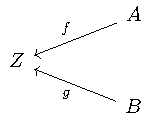
\includegraphics[height=2mm]{assets/images/Chapter_I/3.11a.pdf}}$ is a commutative diagram
        \[\begin{tikzcd}[row sep=0.8em,column sep=2em,ampersand replacement=\&]
            \&\&\& A \ar[dll, "f"] \ar[dlll, swap, bend right, "f"] \\
            Z \& Z \ar[l, swap, "\one_Z"] \\
            \&\&\& B \ar[ull, swap, "g"] \ar[ulll, bend left, "g"]
        \end{tikzcd}\]
        in $\cat{C}$. 
    \end{itemize}
    Then it can be immediately shown that $\cat{C}^{A,B}$ is a category.

    Secondly, we will fix two morphisms $\alpha : C \to A$, $\beta : C \to B$ where $A,B,C$ are fixed objects of $\cat{C}$. We can define a new category $\cat{C}^{\alpha,\beta}$ by essentially the same procedure that we used in order to define $\cat{C}^\alpha$:
    \begin{itemize}[label=$\bullet$]
        \item $\Obj{\cat{C}^{\alpha,\beta}}$ is the collection of all commutative diagrams
        \[\begin{tikzcd}[row sep=0.8em,column sep=2em,ampersand replacement=\&]
            \&\& A \ar[dll, swap, "f"] \\
            Z \&\&\&\& C \ar[dll, "\beta"] \ar[ull, swap, "\alpha"]\\
            \&\& B \ar[ull, "g"]
        \end{tikzcd}\]
        in $\cat{C}$;

        \item morphisms
        \[\begin{tikzcd}[row sep=0.8em,column sep=2em,ampersand replacement=\&]
            \&\& A \ar[dll, swap, "f_1"] \&\& \&\& \&\& A \ar[dll, swap, "f_2"]\\
            Z_1 \&\&\&\& C \ar[dll, "\beta"] \ar[ull, swap, "\alpha"] \ar[rr] \&\& Z_2 \&\&\&\& C \ar[dll, "\beta"] \ar[ull, swap, "\alpha"] \\
            \&\& B \ar[ull, "g_1"] \&\& \&\& \&\& B \ar[ull, "g_2"]
        \end{tikzcd}\]
        are commutative diagrams:
        \[\begin{tikzcd}[row sep=0.8em,column sep=2em,ampersand replacement=\&]
            \& \&\& A \ar[dll, swap, "f_2"] \ar[dlll, swap, bend right, "f_1"] \\
            Z_1 \& Z_2 \ar[l, "\sigma"] \&\&\&\& C \ar[dll, "\beta"] \ar[ull, swap, "\alpha"]\\
            \& \&\& B \ar[ull, "g_2"] \ar[ulll, bend left, "g_1"]
        \end{tikzcd}\]
        in $\cat{C}$;

        \item composition of two morphisms
        $$\begin{array}{ll}
            \begin{tikzcd}[row sep=0.8em,column sep=2em,ampersand replacement=\&]
                \& \&\& A \ar[dll, swap, "f_2"] \ar[dlll, swap, bend right, "f_1"] \\
                Z_1 \& Z_2 \ar[l, "\sigma"] \&\&\&\& C \ar[dll, "\beta"] \ar[ull, swap, "\alpha"]\\
                \& \&\& B \ar[ull, "g_2"] \ar[ulll, bend left, "g_1"]
            \end{tikzcd}, &
            \begin{tikzcd}[row sep=0.8em,column sep=2em,ampersand replacement=\&]
                \& \&\& A \ar[dll, swap, "f_3"] \ar[dlll, swap, bend right, "f_2"] \\
                Z_2 \& Z_3 \ar[l, "\tau"] \&\&\&\& C \ar[dll, "\beta"] \ar[ull, swap, "\alpha"]\\
                \& \&\& B \ar[ull, "g_3"] \ar[ulll, bend left, "g_2"]
            \end{tikzcd}
        \end{array}$$
        is a commutative diagram
        \[\begin{tikzcd}[row sep=0.8em,column sep=2em,ampersand replacement=\&]
            \& \&\& A \ar[dll, swap, "f_3"] \ar[dlll, swap, bend right, "f_1"] \\
            Z_1 \& Z_3 \ar[l, "\tau\sigma"] \&\&\&\& C \ar[dll, "\beta"] \ar[ull, swap, "\alpha"]\\
            \& \&\& B \ar[ull, "g_3"] \ar[ulll, bend left, "g_1"]
        \end{tikzcd}\]
        in $\cat{C}$; and

        \item an identity morphism $\one_{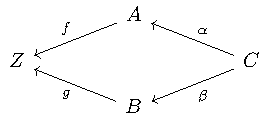
\includegraphics[height=2mm]{assets/images/Chapter_I/3.11b.pdf}}$ is a commutative diagram
        \[\begin{tikzcd}[row sep=0.8em,column sep=2em,ampersand replacement=\&]
            \& \&\& A \ar[dll, swap, "f"] \ar[dlll, swap, bend right, "f"] \\
            Z \& Z \ar[l, "\one_Z"] \&\&\&\& C \ar[dll, "\beta"] \ar[ull, swap, "\alpha"]\\
            \& \&\& B \ar[ull, "g"] \ar[ulll, bend left, "g"]
        \end{tikzcd}\]
        in $\cat{C}$.
    \end{itemize}
    Then it can be quite easily shown that $\cat{C}^{\alpha,\beta}$ is a category.
}

\newpage
\section{Morphisms}
\problem{
    $\vartriangleright$ composition is defined for \emph{two} morphisms. If more than two morphisms are given, e.g.,
    \begin{cd}
        A \ar[r, "f"] \& B \ar[r, "g"] \& C \ar[r, "h"] \& D \ar[r, "i"] \& E,
    \end{cd}
    then one may compose them in several ways, for example:
    \[\begin{array}{llll}(ih)(gf), & (i(hg))f, & i((hg)f), & \text{etc.} \end{array}\]
    so that at every step one is only composing two morphisms. Prove that the result of any such nested composition is independent of the placement of the parantheses. (Hint: Use induction on $n$ to show that any such choice for $f_n f_{n-1} \cdots f_1$ equals
    \[((\cdots((f_n f_{n-1})f_{n-2})\cdots)f_1).\]
    Carefully working out the case $n=5$ is helpful.) \(\left[\text{\S4.1, \S II.1.3}\right]\)
}{
    If $n \leq 4$, then it is obvious that any such choices for $f_n f_{n_1} \cdots f_1$ are equal to $((\cdots((f_n f_{n-1})f_{n-2})\cdots f_2)f_1)$.
    
    Now assume that any such choices for $f_n f_{n-1} \cdots f_1$ are equal to $((\cdots((f_n f_{n-1})f_{n-2})\cdots f_2)f_1)$ for $n \leq k$. Then it is obvious that $((f_{k+1}f_k \cdots f_2)f_1) = ((\cdots((f_{k+1} f_k)f_{k-1})\cdots f_2)f_1)$.

    Now consider the case that $((f_{k+1} f_k \cdots f_{m+1})(f_m f_{m-1} \cdots f_1))$. By the associativity of composition, $((f_{k+1} f_k \cdots f_{m+1})(f_m f_{m-1} \cdots f_1)) = ((f_{k+1} f_k \cdtos f_{m+1})((f_m f_{m-1} \cdots f_2)f_1)) = (((f_{k+1}f_k \cdots f_{m+1})(f_m f_{m-1} \cdots f_2))f_1) = ((f_{k+1} f_k \cdots f_2)f_1) = ((\cdots((f_{k+1}f_k)f_{k-1})\cdots f_2)f_1)$.

    Thus, any such choices for $f_{k+1}f_k \cdots f_1$ are equal to $((\cdots ((f_{k+1}f_k)f_{k-1})\cdots f_2)f_1)$. Therefore, by the induction, the statement is proved.
}

\problem{
    $\vartriangleright$ In Example 3.3 we have seen how to construct a category from a set endowed with a relation, provided this latter is reflexive and transitive. For what types of relations is the corresponding category a groupoid (cf. Example 4.6)? \(\left[ \text{\S4.1} \right]\)
}{
    Let $S$ be a set endowed a relation $\mathrel{\mathcal{R}}$, and $\mathrel{\mathcal{R}}$ be reflexive and transitive. Now let $\hat{S}$ be a category corresponding to $(S,\mathrel{\mathcal{R}})$ and consider a morphism $f : A \to B$ in $\hat{S}$.
    
    If $f$ is an isomorphism, then there exists an inverse $f^{-1} : B \to A$ and this means that $B \mathrel{\mathcal{R}} A$. Hence, if $\hat{S}$ is a groupoid, then every morphism in $\hat{S}$ is an isomorphism, and thus the relation $\mathrel{\mathcal{R}}$ on the set $S$ is symmetric.

    Furthermore, if the relation $\mathrel{\mathcal{R}}$ is symmetric, then it is immediately verified that $\hat{S}$ is a groupoid. Therefore, every category, which is a groupoid, is corresponding to an equivalence relation.
}
\chapter{Groups, first encounter}
\section{Definition of group}
\problem{ %1.1
    $\vartriangleright$ Write a careful proof that every group is the group of isomorphisms of a groupoid. In particular, every group is the group of automorphisms of some object in some category. \sqref{\S2.1}
}{
    Let a group $(G,\cdot)$ be given.

    Now consider a single object category $\cat{C}$ which satisfies that $\Obj{\cat{C}} = \{ \cdot \}$, $\End{\cat{C}}{\cdot} = G$, and the composition of morphisms defined as $gf := g \cdot f$ in.
    
    Then it is obvious that $\cat{C}$ is a groupoid because every morphism has inverse since $gg^{-1} = g^{-1}g = \one$.

    Therefore, every group is the group of isomorphism of a groupoid and the rest of the exercise is completed.
}

\problem{ %1.2
    $\vartriangleright$ Consider the `sets of numbers' listed in \S1.1, and decide which are made into groups by conventional operations such as $+$ and $\cdot$. Even if the answer is negative (for example, $(\RR,\cdot)$ is not a group), see if variations on the definition of these sets lead to groups (for example, $(\RR^*,\cdot)$ \emph{is} a group; cf. \S1.4). \sqref{\S1.2}
}{
    \begin{itemize}[leftmargin=51mm]
        \item[\textbf{Groups}] $(\ZZ,+)$, $(\QQ,+)$, $(\RR,+)$, $(\CC,+)$

        \item[\textbf{Non-groups}] $(\NN,+)$, $(\NN,\cdot)$, $(\ZZ,\cdot)$, $(\QQ,\cdot)$, $(\RR,\cdot)$, $(\CC,\cdot)$

        \item[\textbf{Variations which are groups}] $(\QQ^*,\cdot)$, $(\QQ^+,\cdot)$, $(\RR^*,\cdot)$, $(\RR^+,\cdot)$, $(\CC^*,\cdot)$
    \end{itemize}
}
\clearpage

\problem{ %1.3
    Prove that $(gh)^{-1} = h^{-1}g^{-1}$ for all elements $g$, $h$ of a group $G$.
}{
    $(h^{-1}g^{-1})(gh) = \left( h^{-1} (g^{-1}g) \right) h = (h^{-1}e)h = h^{-1}h = e$.
    $(gh)(h^{-1}g^{-1}) = \left( g (hh^{-1}) \right) g^{-1} = (ge)g^{-1} = gg^{-1} = e$.
    Since the inverse of $gh$ is unique, $h^{-1}g^{-1}$ is the inverse of $gh$.
}

\problem{ %1.4
    Suppose that $g^2 = e$ for all elements $g$ of a group $G$; prove that $G$ is commutative.
}{
    Let $g$ be an element of $G$. Then $g = g^{-1}$ since $gg = e$.

    Now let $h$ also be an element of $G$. Then $gh = (gh)^{-1} = h^{-1}g^{-1} = hg$ since $G$ is a group.

    Therefore, $G$ is commutative.
}

\problem{ %1.5
    The `multiplication table' of a group is an array compiling the results of all multiplications $g \bullet h$:
    \begin{center}
        \begin{tabular}{c||c|c|c|c}
            $\bullet$ & $e$ & $\cdots$ & $h$ & $\cdots$ \\ \hline\hline
            $e$ & $e$ & $\cdots$ & $h$ & $\cdots$ \\ \hline
            $\cdots$ & $\cdots$ & $\cdots$ & $\cdots$ & $\cdots$ \\ \hline
            $g$ & $g$ & $\cdots$ & $g \bullet h$ & $\cdots$ \\ \hline
            $\cdots$ & $\cdots$ & $\cdots$ & $\cdots$ & $\cdots$
        \end{tabular}
    \end{center}
    (Here $e$ is the identity element. Of course the table depends on the order in which the elements are listed in the top row and leftmost column.) Prove that every row and every column of the multiplication table of a group contains all elements of the group exactly once (like Sudoku diagrams!).
}{
    Let $l_g : G \to G$ be a function defined as $l_g : x \mapsto gx$ for each $g \in G$.
    
    Then it is clear that $l_g$ is surjective since $l_g(g^{-1}x) = x$ for any $x \in G$, and it is obvious that $l_g$ is injective since $l_g(x) = l_g(y)$ implies that $x = g^{-1}l_g(x) = g^{-1}l_g(y) = y$ for any $x,y \in G$.

    Hence, $l_g$ is a bijection and this means that each row of the multiplication table of a group contains every element of the group exactly once.

    Similarly, it is readily shown that each column of the multiplication table of a group contains every element of the group exactly once.
}

\problembr{ %1.6
    $\neg$ Prove that there is only \emph{one} possible multiplication table for $G$ if $G$ has exactly 1, 2, or 3 elements. Analyze the possible multiplication tables for groups with exactly 4 elements, and show that there are \emph{two} distinct tables, up to reordering the elements of $G$. Use these tables to prove that all groups with $\leq$ 4 elements are commutative.\\ \indent (You are welcome to analyze groups with 5 elements using the same technique, but you will soon know enough about groups to be able to avoid such brute-force approaches.) \sqref{2.19}
}{
    If $G$ has only one element, then the binary operation $\cdot : G \times G \to G$ is unique and the multiplication table has to be the below one:
    \begin{center}
        \begin{tabular}{c||c}
            $\cdot$ & $e$ \\ \hline\hline
            $e$ & $e$
        \end{tabular}
    \end{center}

    If $G$ has only two element $e$,$a$, then it has to be $ee = e$ and $ae = ea = a$. In the case that $aa = a$, then $a$ has no inverse so it has to be $aa = e$. Thus, the multiplication table of $G$ has to be the below one:
    \begin{center}
        \begin{tabular}{c||c|c}
            $\cdot$ & $e$ & $a$ \\ \hline\hline
            $e$ & $e$ & $a$ \\ \hline
            $a$ & $a$ & $e$
        \end{tabular}
    \end{center}

    Now consider the case that $G$ has exactly 3 elements, $e$, $a$, $b$. Then it is obvious that $ee = e$, $ea = ae = a$, $eb = be = b$. Since every element of a group has an inverse, it has to be either $a^2 = b^2 = e$ or $ab = ba = e$.
    
    In the case of $a^2 = b^2 = e$, $ab = b$ since the function $G \to G : x \mapsto ax$ is bijective. But by cancellation, $ab = b$ induces the fact that $a = e$, and this contradicts the fact that $e$, $a$, $b$ are distinct. 
    
    Hence, we can obtain $ab = ba = e$ and this means that $a^2 = b$ and $b^2 = a$ since each row of the multiplication table contains $e$, $a$, $b$ exactly once. To sum up, the multiplication table has to be the below one:
    \begin{center}
        \begin{tabular}{c||c|c|c}
            $\cdot$ & $e$ & $a$ & $b$ \\ \hline\hline
            $e$ & $e$ & $a$ & $b$ \\ \hline
            $a$ & $a$ & $b$ & $e$ \\ \hline
            $b$ & $b$ & $e$ & $a$
        \end{tabular}
    \end{center}

    Finally, now consider the situation that $G$ has only 4 elements, $e$, $a$, $b$, $c$. Then it is obvious that $ee = e$, $ea = ae = a$, $eb = be = b$, and $ec = ce = c$.

    Since $a$ has an inverse, it has to be either $a^2 = e$ or $ab = ba = e$. The case of $ac = ca = e$ is the same situation with the case of $ab = ba = e$ up to reordering the elements.

    If $a^2 = e$, then it is clear that $ab = ba = c$ and $ac = ca = b$ since each row and column of the multiplication table contains $e$, $a$, $b$, $c$ exactly once.

    Thus, in the case of $a^2 = e$, the multiplication table of $G$ has to be one of the below:
    \begin{center}
        \begin{tabular}{c||c|c|c|c}
            $\cdot$ & $e$ & $a$ & $b$ & $c$ \\ \hline\hline
            $e$ & $e$ & $a$ & $b$ & $c$ \\ \hline
            $a$ & $a$ & $e$ & $c$ & $b$ \\ \hline
            $b$ & $b$ & $c$ & $e$ & $a$ \\ \hline
            $c$ & $c$ & $b$ & $a$ & $e$
        \end{tabular}, \quad \begin{tabular}{c||c|c|c|c}
            $\cdot$ & $e$ & $a$ & $b$ & $c$ \\ \hline\hline
            $e$ & $e$ & $a$ & $b$ & $c$ \\ \hline
            $a$ & $a$ & $e$ & $c$ & $b$ \\ \hline
            $b$ & $b$ & $c$ & $a$ & $e$ \\ \hline
            $c$ & $c$ & $b$ & $e$ & $a$
        \end{tabular}
    \end{center}

    In the case of $ab = ba = e$ is the same case with the second table up to reordering the elements.

    Therefore, the desired results follow.

    Analyzing groups with 5 elements using the same technique requires a lot of effort, and the result is just a fact that there is only one group of order 5, whose multiplication table is just below:
    \begin{center}
        \begin{tabular}{c||c|c|c|c|c}
            $\cdot$ & $e$ & $a$ & $b$ & $c$ & $d$ \\ \hline\hline
            $e$ & $e$ & $a$ & $b$ & $c$ & $d$ \\ \hline
            $a$ & $a$ & $b$ & $c$ & $d$ & $e$ \\ \hline
            $b$ & $b$ & $c$ & $d$ & $e$ & $a$ \\ \hline
            $c$ & $c$ & $d$ & $e$ & $a$ & $b$ \\ \hline
            $d$ & $d$ & $e$ & $a$ & $b$ & $c$
        \end{tabular}
    \end{center}
}

\problem{ %1.7
    Prove Corollary 1.11.
}{
    \begin{itemize}[leftmargin=12mm]
        \item[($\implies$)] This is just the result of Lemma 1.10.

        \item[($\impliedby$)] If $N$ is a multiple of $\abs{g}$, then $N = m\abs{g}$ for some integer $m$. Hence, $g^N = g^{m\abs{g}} = \left( g^{\abs{g}} \right)^m = e^m = e$.
    \end{itemize}
}

\problem{ %1.8
    $\neg$ Let $G$ be a finite abelian group, with exactly one element $f$ of order 2. Prove that $\prod_{g \in G} g = f$. \sqref{4.16}
}{
    Let $H = \{ g \in G \mid \abs{g} > 2 \}$. Then $\prod_{g \in G} g = f \prod_{g \in H} g$, obviously, since $G$ is commutative.
    
    Since $g^{\abs{g}-1} = g^{-1}$ for any $g \in G$, $\prod_{g \in H} g = e$, clearly.

    Therefore, $\prod_{g \in G} g = f$ since $f^{-1} = f$.
}

\problem{ %1.9
    Let $G$ be a finite group, of order $n$, and let $m$ be the number of elements $g \in G$ of order exactly 2. Prove that $n-m$ is odd. Deduce that if $n$ is even, then $G$ necessarily contains elements of order 2.
}{
    If $\abs{g} > 2$, then $g^{-1} \neq g$ since $g^{-1} = g^{\abs{g}-1}$.

    Hence, the subset of $G$ whose elements have order greater than 2 has even elements.

    Therefore, $n-m = 1 + \{ g \in G \mid \abs{g} > 2 \}$ is an odd number.
}

\problem{ %1.10
    Suppose the order of $g$ is odd. What can you say about the order of $g^2$?
}{
    Since $(g^2)^{\abs{g}} = (g^{\abs{g}})^2 = e^2 = e$, $\abs{g^2}$ divides $\abs{g}$.

    Since $g^{2\abs{g^2}} = (g^2)^{\abs{g^2}} = e$, $\abs{g}$ divides $2\abs{g^2}$, and thus $\abs{g}$ divides $\abs{g^2}$ since $\abs{g}$ is odd and by the Euclid's lemma.

    Therefore, $\abs{g} = \abs{g^2}$ since $\abs{g}$ and $\abs{g^2}$ are greater than 0.
}

\problem{ %1.11
    Prove that for all $g$, $h$ in a group $G$, $\abs{gh} = \abs{hg}$. (Hint: Prove that $\abs{aga^{-1}} = \abs{g}$ for all $a,$ $g$ in $G$.)
}{
    $$\begin{array}{rcl}
        (aga^{-1})^n = e & \iff & ag^na^{-1} = e \\
        & \iff & ag^n = a \\
        & \iff & g^n = e \text{ for any } a,g \in G.
    \end{array}$$

    Thus, it is clear that $\abs{g} = \abs{aga^{-1}}$ and this implies that $\abs{gh} = \abs{h(gh)h^{-1}} = \abs{hg}$.
}

\problem{ %1.12
    $\vartriangleright$ In the group of invertible $2 \times 2$ matrices, consider
    $$g = \mat{0 & -1 \\ 1 & 0}, h = \mat{0 & 1 \\ -1 & -1}.$$
    Verify that $\abs{g} = 4$, $\abs{h} = 3$, and $\abs{gh} = \infty$. \sqref{\S1.6}
}{
    Since $g^4 = I$ and $g^2 = -I$, $\abs{g} = 4$.

    Since $h^3 = I$ and 3 is a prime, $\abs{h} = 3$.

    Now consider the $gh = \mat{1 & 1 \\ 0 & 1}$.

    Since $\mat{1 & 1 \\ 0 & 1}^n = \mat{1 & n \\ 0 & 1}$, $\abs{gh} = \infty$.
}

\problem{ %1.13
    $\vartriangleright$ Give an example showing that $\abs{gh}$ is not necessarily equal to $\lcm (\abs{g},\abs{h})$, even if $g$ and $h$ commute. \sqref{\S1.6, 1.14}
}{
    Let $h = g^{-1}$. Then $\abs{gh} = 1$ and $gh = hg$.
}

\problem{ %1.14
    $\vartriangleright$ As a counterpoint to \ref{prob:II.1.13}, prove that if $g$ and $h$ commute \emph{and} $\gcd(\abs{g},\abs{h}) = 1$, then $\abs{gh} = \abs{g}\abs{h}$. (Hint: Let $N = \abs{gh}$; then $g^N = (h^{-1})^N$. What can you say about this element?) \sqref{\S1.6, 1.15, \S IV.2.5}
}{
    Since $gh = hg$, $(gh)^{\abs{gh}} = g^{\abs{gh}}h^{\abs{gh}}$.

    Thus, $g^{\abs{gh}} = (h^{-1})^{\abs{gh}}$ and this implies that $(h^{-1})^{\abs{g}\abs{gh}} = e$. Hence, $\abs{h}$ divides $\abs{g}\abs{gh}$.

    Since $\gcd (\abs{g},\abs{h}) = 1$, by Euclid's lemma, $\abs{h}$ divides $\abs{gh}$.

    In the same way, we can get the fact that $\abs{g}$ divides $\abs{gh}$ and so we get $\abs{g}\abs{h}$ divides $\abs{gh}$ since $\lcm (\abs{g},\abs{h}) = \abs{g}\abs{h}$.

    Moreover, $(gh)^{\abs{g}\abs{h}} =g^{\abs{g}\abs{h}}h^{\abs{g}\abs{h}} = e^{\abs{h}}e^{\abs{g}} = e$ and this means that $\abs{gh}$ divides $\abs{g}\abs{h}$.

    Therefore, $\abs{gh} = \abs{g}\abs{h}$.
}

\problem{ %1.15
    $\neg$ Let $G$ be a commutative group, and let $g \in G$ be an element of maximal \emph{finite} order, that is, such that if $h \in G$ has finite order, then $\abs{h} \leq \abs{g}$. Prove that in fact if $h$ has finite order in $G$, then $\abs{h}$ \emph{divides} $\abs{g}$. (Hint: Argue by contradiction. If $\abs{h}$ is finite but does not divide $\abs{g}$, then there is a prime integer $p$ such that $\abs{g} = p^mr$, $\abs{h} = p^ns$, with $r$ and $s$ relatively prime to $p$ and $m < n$. Use \ref{prob:II.1.14} to compute the order of $g^{p^m}h^s$.) \sqref{\S2.1, 4.11, IV.6.15}
}{
    Suppose not, i.e., $\abs{h}$ is finite but $\abs{h}$ does not divide $\abs{g}$.

    Then there is a prime number $p$ such that $\abs{g} = p^mr$, $\abs{h} = p^ns$, $p \nmid r$, $p \nmid s$, and $m < n$.

    Then by the result of \ref{prob:II.1.14}, $\abs{g^{p^m}h^s} = p^nr > p^mr = \abs{g}$ and this contradicts the maximality of $g$.

    Therefore, the desired result is shown.
}

\newpage
\section{Examples of groups}
\problem{ %2.1
    $\neg$ One can associate an $n \times n$ matrix $M_\sigma$ with a permutation $\sigma \in S_n$ by letting the entry at $(i,(i)\sigma)$ be 1 and letting all other entries be 0. For example, the matrix corresponding to the permutation
    $$ \sigma = \mat{1 & 2 & 3 \\ 3 & 1 & 2} \in S_3 $$
    would be
    $$ M_\sigma = \mat{0 & 0 & 1 \\ 1 & 0 & 0 \\ 0 & 1 & 0}. $$
    Prove that, with this notation,
    $$ M_{\sigma\tau} = M_\sigma M_\tau $$
    for all $\sigma,\tau \in S_n$, where the product on the right is the ordinary product of matrices. \sqref{IV.4.13}
}{
    Since $M_\sigma = \bmat{ \delta_{(i)\sigma,j} }_{n \times n}$,
    $\begin{array}{rl}
        M_\sigma M_\tau & = \bmat{ \delta_{(i)\sigma,j} }_{n \times n} \bmat{ \delta_{(i)\tau,j} }_{n \times n} \\
        & = \bmat{ \sum_{k=1}^n \delta_{(i)\delta,k} \delta_{(k)\tau,j} }_{n \times n} \\
        & = \bmat{ \delta_{((i)\sigma)\tau,j} }_{n \times n} \\
        & = \bmat{ \delta_{(i)(\sigma\tau),j} }_{n \times n} \\
        & = M_{\sigma\tau}
    \end{array}$.
}

\problem{ %2.2
    $\vartriangleright$ Prove that if $d \leq n$, then $S_n$ contains elements of order $d$. \sqref{\S2.1}
}{
    $\mat{1 & 2 & \cdots & d-1 & d & d+1 & d+2 & \cdots & n \\ 2 & 3 & \cdots & d & 1 & d+1 & d+2 & \cdots & n} \in S_n$ has the order $d$.
}

\problem{ %2.3
    For every positive integer $n$ find an element of order $n$ in $S_\NN$.
}{
    The order of the cycle $\mat{1 & 2 & 3 & \cdots & n} \in S_{\NN}$ is $n$.
}

\problembr{ %2.4
    Define a homomorphism $D_8 \to S_4$ by labeling vertices of a square, as we did for a triangle in \S2.2. List the 8 permutations in the image of this homomorphism.
    \clearpage
}{
    Label the vertices of a square like below:\\
    \adjustbox{scale=0.5,center}{
        \begin{tikzcd}[ampersand replacement=\&]
            \scalebox{2}{1} \ar[rrr,no head,shift right=4,shorten >= 0pt,shorten <= 0pt] \&\&\& \scalebox{2}{2} \ar[ddd,no head,shift right=4,shorten >= 3pt,shorten <= 3pt] \\ \\ \\
            \scalebox{2}{4} \ar[uuu,no head,shift right=4,shorten >= 3pt,shorten <= 3pt] \&\&\& \scalebox{2}{3} \ar[lll,no head,shift right=7,shorten >= 0pt,shorten <= 0pt]
        \end{tikzcd}
    }
    
    Then, the image of the homomorphism consists of
    $$\mat{1 & 2 & 3 & 4 \\ 1 & 2 & 3 & 4}, \mat{1 & 2 & 3 & 4 \\ 2 & 3 & 4 & 1}, \mat{1 & 2 & 3 & 4 \\ 3 & 4 & 1 & 2}, \mat{1 & 2 & 3 & 4 \\ 4 & 1 & 2 & 3},$$
    $$\mat{1 & 2 & 3 & 4 \\ 4 & 3 & 2 & 1}, \mat{1 & 2 & 3 & 4 \\ 2 & 1 & 4 & 3}, \mat{1 & 2 & 3 & 4 \\ 3 & 2 & 1 & 4}, \mat{1 & 2 & 3 & 4 \\ 1 & 4 & 3 & 2}.$$
}

\problem{ %2.5
    $\vartriangleright$ Describe generators and relations for all dihedral groups $D_{2n}$. (Hint: Let $x$ be the reflection about a line through the center of a regular $n$-gon and a vertex, and let $y$ be the counterclockwise rotation by $2\pi/n$. The group $D_{2n}$ will be generated by $x$ and $y$, subject to three relations. To see that these relations really determine $D_{2n}$, use them to show that any product $x^{i_1}y^{i_2}x^{i_3}y^{i_4}\cdots$ equals $x^iy^j$ for some $i$, $j$ with $0 \leq i \leq 1$, $0 \leq j < n$.) \sqref{8.4, \S IV.2.5}
}{
    Let $x$ be the reflection about a line through the center of a regular $n$-gon and a vertex, and let $y$ be the counterclockwise rotation by $2\pi/n$. Then we can find relations $x^2 = e$, $y^n = e$, $yx = xy^{n-1}$. These relations hold indeed and we have to show that the other relations are not needed to determine $D_{2n}$.

    We can easily observe that any product $x^{i_1}y^{i_2}x^{i_3}y^{i_4}\cdots$ can be reduced as $x^iy^j$ for some $i,j$ with $0 \leq i \leq 1$ and $0 \leq j < n$ since $yxy = xy^{n-1}y = x$, and $xyx = xxy^{n-1} = y^{n-1}$.

    Therefore, $D_{2n} = \left< x,y \mid x^2 = y^n = e, yx = xy^{n-1} \right>$.
}

\problem{ %2.6
    $\vartriangleright$ For every positive integer $n$ construct a group containing elements $g$, $h$ such that $\abs{g} = 2$, $\abs{h} = 2$, and $\abs{gh} = n$. (Hint: For $n > 1$, $D_{2n}$ will do.) \sqref{\S1.6}
}{
    For $n = 1$, we can take $\ZZ_2$. If we take $g = h = 1$, then $\abs{g} = \abs{h} = 2$ and $\abs{gh} = 1$.

    For $n > 1$, we can take $D_{2n}$. Let $x$ be the reflection about a line through the center of a regular $n$-gon and a vertex, and let $y$ be the counterclockwise rotation by $2\pi/n$. Then, $\abs{x} = \abs{xy} = 2$ and $\abs{y} = n$. Hence, we can take $g = x$ and $h = xy$.
}

\problembr{ %2.7
    Find all elements of $D_{2n}$ that commute with every other element.
    (The parity of $n$ plays a role.)
    \clearpage
}{
    Let $x$ be the reflection about a line through the center of a regular $n$-gon and a vertex, and let $y$ be the counterclockwise rotation by $2\pi/n$.
    
    Then by the result of \ref{prob:II.2.5}, every element of $D_{2n}$ can be written as $x^i y^j$ with $0 \leq i \leq 1$ and $0 \leq j < n$, and distinct representations represent distinct elements.
    
    Now consider two elements $x^{i_1} y^{j_1}$ and $x^{i_2} y^{j_2}$. Then $x^{i_1}y^{j_1}x^{i_2}y^{j_2} = x^{i_1+i_2} y^{(-1)^{i_2}j_1+j_2}$. So if these commute with each other, then $(-1)^{i_2} j_1 + j_2 \equiv (-1)^{i_1} j_2 + j_1 \pmod{n}$.

    Hence, if $n$ is odd, $e$ is the only element that commutes with every other element, and otherwise, $e$ and $y^{n/2}$ are the only elements that commute with every other element.
}

\problem{ %2.8
    Find the orders of the groups of symmetries of the five `platonic solids'.
}{
    Let $T$, $C$, $O$, $D$, $I$ be the respective groups of symmetries of the regular tetrahedron, cube, regular octahedron, regular dodecahedron, and regular icosahedron.

    Then $\abs{T} = 4 \times \abs{D_6} = 24$, $\abs{O} = 6 \times \abs{D_8} = 48$, and $\abs{I} = 12 \times \abs{D_{10}} = 120$, obviously.

    Furthermore, since the cube is a dual polyhedron of the regular octahedron, and since the regular dodecahedron is a dual polyhedron of the regular icosahedron, $O$ is isomorphic to $C$ and $I$ is isomorphic to $D$. Thus, $\abs{C} = \abs{O} = 48$ and $\abs{D} = \abs{I} = 120$.
}

\problem{ %2.9
    Verify carefully that `congruence mod $n$' is an equivalence relation.
}{
    Note that $a \equiv b \pmod{n}$ if and only if $n \mid a-b$.

    Since $n \mid 0$, $a \equiv a \pmod{n}$ for any $a \in \ZZ$ and thus the relation `congruence mod $n$' is reflexive.

    Since $n \mid x$ implies that $n \mid -x$, $a \equiv b \pmod{n}$ implies $b \equiv a \pmod{n}$ for any $a,b \in \ZZ$ and thus the relation `congruence mod $n$' is symmetric.

    Since $n \mid x$ and $n \mid y$ imply that $n \mid x+y$, $a \equiv b \pmod{n}$ and $b \equiv c \pmod{n}$ imply $a \equiv c \pmod{n}$ for any $a,b,c \in \ZZ$ and thus the relation `congruence mod $n$' is transitive.

    Therefore, the relation `congruence mod $n$' is an equivalence relation.
}

\problem{ %2.10
    Prove that if $n > 0$, then $\ZZ / n\ZZ$ consists of precisely $n$ elements.
}{
    Let $0 \leq i < j < n$ and $i \equiv j \pmod{n}$. Then $n \mid j-i$ and since $0 < j-i < n$, it immediately makes a contradiction. Hence, for any $0 \leq i < j < n$, $[i] \neq [j]$. This means that $\abs{\cyclic{n}} \geq n$.

    Now, for any integer $m$, by the division theorem, there are integers $q,r$ such that $m = qn+r$ and $0 \leq r < n$. Hence, $[m] = [r]$ for some $0 \leq r < n$, and this means that $\abs{\cyclic{n}} \leq n$.

    Therefore, $\ZZ / n\ZZ$ consists of precisely $n$ elements.
}

\problem{ %2.11
    $\vartriangleright$ Prove that the square of every odd integer is congruent to 1 modulo 8. \sqref{\S VII.5.1}
}{
    Since $(4k \pm 1)^2 = 16k^2 \pm 8k + 1 = 8(2k^2 \pm k) + 1$, the square of every odd integer is congruent to 1 modulo 8.
}

\problem{ %2.12
    Prove that there are no nonzero integers $a$, $b$, $c$ such that $a^2 + b^2 = 3c^2$. (Hint: By studying the equation $[a]_4^{\phantom{4}2} + [b]_4^{\phantom{4}2} = 3[c]_4^{\phantom{4}2}$ in $\cyclic{4}$, show that $a,b,c$ would all have to be even. Letting $a = 2k$, $b = 2l$, $c = 2m$, you would have $k^2 + l^2 = 3m^2$. What's wrong with that?)
}{
    Let $a^2 + b^2 = 3c^2$ for some integers $a$, $b$, $c$. Then $a^2 + b^2 \equiv 3c^2 \pmod{4}$, clearly.

    If $c$ is odd, then $3c^2 \equiv 3 \pmod{4}$ and this makes a contradiction since the square of every integer is congruent to 0 or 1 modulo 4.

    Thus, $c$ is even, and this implies that $a$ and $b$ are also even by the same reason above.

    Hence, $a = b = c = 0$, obviously since $a^2 + b^2 = 3c^2 \implies (\tfrac{a}{2})^2 + (\tfrac{b}{2})^2 = 3(\tfrac{c}{2})^2$.
}

\problem{ %2.13
    $\vartriangleright$ Prove that if $\gcd (m,n) = 1$, then there exist integers $a$ and $b$ such that
    $$ am + bn = 1. $$
    (Use Corollary 2.5.) Conversely, prove that if $am + bn = 1$ for some integers $a$ and $b$, then $\gcd (m,n) = 1$. \sqref{2.15, \S V.2.1, V.2.4}
}{
    If $\gcd (m,n) = 1$, by Corollary 2.5, $[m]_n$ generates $\ZZ / n\ZZ$, and this means that $km \equiv 1 \pmod{n}$ for some integer $k$, so there exist integers $a,b$ such that $am + bn = 1$.

    If $am + bn = 1$ for some integers $a,b$, then $\gcd (m,n) \mid 1$, obviously, and this means that $\gcd (m,n) = 1$.
}

\problem{ %2.14
    $\vartriangleright$ State and prove an analog of Lemma 2.2, showing that the multiplication on $\ZZ / n\ZZ$ is a well-defined operation. \sqref{\S2.3, \S III.1.2}
}{
    ``$a_1 \equiv a_2 \pmod{n}$ and $b_1 \equiv b_2 \pmod{n}$ implies that $a_1b_1 \equiv a_2b_2 \pmod{n}$.''

    Since $a_1 \equiv a_2 \pmod{n} \iff \exists k \in \ZZ \st a_1 - a_2 = kn$ and $b_1 \equiv b_2 \pmod{n} \iff \exists l \in \ZZ \st b_1 - b_2 = ln$, $a_1 \equiv a_2 \pmod{n}$ and $b_1 \equiv b_2 \pmod{n}$ implies that $a_1b_1 - a_2b_2 = a_1(b_1-b_2) + b_2(a_1-a_2) = a_1ln + b_2kn = (a_1l+b_2k)n$ and this immediately gives us $a_1b_1 \equiv a_2b_2 \pmod{n}$.
}

\problem{ %2.15
    $\neg$ Let $n > 0$ be an odd integer.

    \begin{itemize}[label=$\bullet$]
        \item Prove that if $\gcd (m,n) = 1$, then $\gcd (2m+n,2n) = 1$. (Use \ref{prob:II.2.13}.)

        \item Prove that if $\gcd (r,2n) = 1$, then $\gcd (\tfrac{r-n}{2},n) = 1$. (Ditto.)

        \item Conclude that the function $[m]_n \to [2m+n]_{2n}$ is a bijection between $(\cyclic{n})^*$ and $(\cyclic{2n})^*$.
    \end{itemize}
    The number $\phi(n)$ of elements of $(\cyclic{n})^*$ is \emph{Euler's $\phi$-function}. The reader has just proved that if $n$ is odd, then $\phi(2n) = \phi(n)$. Much more general formulas will be given later on (cf. \ref{exer:V.6.8}). \sqref{VII.5.11}
}{
    Since $2 \nmid 2m+n$, $\gcd (2m+n,2n) = \gcd (2m+n,n) = \gcd (2m,n)$.

    Since $2 \nmid n$, $\gcd (2m,n) = \gcd(m,n)$.

    Since $2 \nmid n$, $\gcd (\tfrac{r-n}{2},n) = \gcd (r-n,n) = \gcd (r,n)$.

    By the above, $[m]_n \mapsto [2m+n]_{2n}$ is bijection between $(\ZZ / n\ZZ)^*$ and $(\ZZ / 2n\ZZ)^*$, obviously.
}

\problem{ %2.16
    Find the last digit of $1238237^{18238456}$. (Work in $\cyclic{10}$.)
}{
    Since $\phi(10) = 4$, $a^5 = a \pmod{10}$ for any integers $a$.

    Hence, $1238237^{18238456} \equiv 7^4 \equiv 1 \pmod{10}$.

    Therefore, the desired answer is 1.
}

\problem{ %2.17
    $\vartriangleright$ Show that if $m \equiv m' \bmod{n}$, then $\gcd (m,n) = 1$ if and only if $\gcd (m',n) = 1$. \sqref{\S2.3}
}{
    By Euclidean algorithm, it is quite obvious.
}

\problem{ %2.18
    For $d \leq n$, define an injective function $\ZZ / d\ZZ \to S_n$ preserving the operation, that is, such that the sum of equivalence classes in $\ZZ / d\ZZ$ corresponds to the product of the corresponding permutations.
}{
    $[m]_d \mapsto \mat{1 & 2 & \cdots & d}^m$ is an injective function $\ZZ / d\ZZ \to S_n$ preserving the operation.
}

\problem{ %2.19
    $\vartriangleright$ Both $(\cyclic{5})^*$ and $(\cyclic{12})^*$ consist of 4 elements. Write their multiplication tables, and prove that no re-ordering of the elements will make them match. (Cf. \ref{prob:II.1.6}.) \sqref{\S4.3}
}{
    The below one is the multiplication table of $(\ZZ / 5\ZZ)^*$.
    \begin{center}
        \begin{tabular}{c||c|c|c|c}
            $\cdot$ & 1 & 2 & 3 & 4 \\ \hline\hline
            1 & 1 & 2 & 3 & 4 \\ \hline
            2 & 2 & 4 & 1 & 3 \\ \hline
            3 & 3 & 1 & 4 & 2 \\ \hline
            4 & 4 & 3 & 2 & 1
        \end{tabular}
    \end{center}

    The below one is the multiplication table of $(\ZZ / 12\ZZ)^*$.
    \begin{center}
        \begin{tabular}{c||c|c|c|c}
            $\cdot$ & 1 & 5 & 7 & 11 \\ \hline\hline
            1 & 1 & 5 & 7 & 11 \\ \hline
            5 & 5 & 1 & 11 & 7 \\ \hline
            7 & 7 & 11 & 1 & 5 \\ \hline
            11 & 11 & 7 & 5 & 1
        \end{tabular}
    \end{center}

    In $(\ZZ / 5\ZZ)^*$, $\abs{2} = 4$. However, there is no element in $(\ZZ / 12\ZZ)^*$, whose order is 4. Therefore, there is no re-ordering of the elements making them match.
}

\newpage
\markboth{\MakeUppercase{Chapter II. Groups, first encounter}}{3. \MakeUppercase{The category} \textsf{Grp}}
\section{The category \textsf{Grp}}
\markboth{\MakeUppercase{Chapter II. Groups, first encounter}}{3. \MakeUppercase{The category} \textsf{Grp}}
\problem{ %3.1
    $\vartriangleright$ Let $\varphi : G \to H$ be a morphism in category $\cat{C}$ with products. Explain why there is unique morphism $(\varphi \times \varphi) : G \times G \to H \times H$ compatible in the evident way with the natural projections.
    
    (This morphism is defined explicitly for $\cat{C} = \Set$ in \S3.1.) \sqref{\S3.1, 3.2}
}{
    \begin{cd}[row sep=0.8em,column sep=4em]
        \&\& H \ar[dll, "\varphi \pi_{G_1}", swap, bend right, <-] \ar[dl, "\pi_{H_1}", swap, <-] \\
        G \times G \& H \times H \ar[l, "\varphi \times \varphi", swap, <-, dashed] \\
        \&\& H \ar[ull, "\varphi \pi_{G_2}", bend left, <-] \ar[ul, "\pi_{H_2}", <-]
    \end{cd}
    
    By the definition of the product $H \times H$, there is a unique morphism $\varphi \times \varphi : G \times G \to H \times H$, which makes the diagram above commute.

    Further, this $\varphi \times \varphi$ is compatible with the natural projections, indeed.
}

\problem{ %3.2
    Let $\varphi : G \to H$, $\psi : H \to K$ be morphisms in a category with products, and consider morphisms between the products $G \times G$, $H \times H$, $K \times K$ as in \ref{prob:II.3.1}. Prove that
    $$ (\psi\varphi) \times (\psi\varphi) = (\psi \times \psi)(\varphi \times \varphi). $$
    (This is part of the commutativity of the diagram displayed in \S3.2.)
}{
    \[\scaledcd{scale=0.7}{
        G \ar[d, "\pi_{G_1}", swap, <-] \ar[r, "\varphi", swap] \ar[rr, "\psi\varphi", bend left, swap] \& H \ar[d, "\pi_{H_1}"{pos=0.4}, <-] \ar[r, "\psi", swap] \& K \ar[d, "\pi_{K_1}", swap, <-] \\
        G \times G \ar[r, "\varphi \times \varphi", swap] \ar[rr, "(\psi\varphi) \times (\psi\varphi)"{pos=0.32}, bend left=20pt] \& H \times H \ar[r, "\psi \times \psi", swap] \& K \times K \\
        G \ar[u, "\pi_{G_2}", <-] \ar[r, "\varphi"] \ar[rr, "\psi\varphi", bend right] \& H \ar[u, "\pi_{H_2}", <-] \ar[r, "\psi"] \& K \ar[u, "\pi_{K_2}", <-]
    }[row sep=4em,column sep=4em]\]
    By the commutativity of the diagram above, $(\psi \times \psi)(\varphi \times \varphi) = (\psi\varphi) \times (\psi\varphi)$.
}

\problembr{ %3.3
    $\vartriangleright$ Show that if $G$, $H$ are \emph{abelian} groups, then $G \times H$ satisfies the universal property for coproducts in $\Ab$ (cf. \S I.5.5). \sqref{\S3.5, 3.6, \S III.6.1}
    \clearpage
}{
    Let $\iota_G : G \to G \times H$ and $\iota_H : H \to G \times H$ be defined as $\iota_G : g \mapsto (g,e_H)$ and $\iota_H : h \mapsto (e_G,h)$, respectively. Now consider an abelian group $K$ and two homomorphisms $\varphi : G \to K$ and $\psi : H \to K$.

    \begin{cd}[row sep=0.8em,column sep=4em]
        \&\& G \ar[dll, "\varphi", bend right, swap] \ar[dl, "\iota_G", swap] \\
        K \& G \times H \ar[l, "\varphi * \psi"{pos=0.33}, swap, dashed] \\
        \&\& H \ar[ull, "\psi", bend left] \ar[ul, "\iota_H"]
    \end{cd}

    To make the diagram above commute, it must be as follows:
    \[\begin{array}{rcl}
        (\varphi * \psi)(g,h) & = & (\varphi * \psi)((g,e_H)(e_G,h)) \\
        & = & (\varphi * \psi)(g,e_H) (\varphi * \psi)(e_G,h) \\
        & = & \varphi(g) \psi(h).
    \end{array}\]

    Therefore, there uniquely exist a homomorphism $\varphi * \psi$ making the diagram above commute and, hence, $G \times H$ satisfies the universal property for coproducts of $G$ and $H$ in $\Ab$.
}

\problem{ %3.4
    Let $G$, $H$ be groups, and assume that $G \cong H \times G$. Can you conclude that $H$ is trivial? (Hint: No. Can you construct a counterexample?)
}{
    Since $\RR$ and $\RR \times \RR$ are vector spaces over the field $\QQ$ with the same dimension, $\RR \cong \RR \times \RR$ as groups.
}

\problem{ %3.5
    Prove that $\QQ$ is not the direct product of two nontrivial groups.
}{
    Suppose not, i.e., $\QQ = G \times H$ for some nontrivial groups $G$ and $H$. Then $G \times \{ e_H \}$ and $\{ e_G \} \times H$ are nontrivial subgroups of $\QQ$ and they have a trivial intersection. But since there exist two integers $n$ and $m$ such that $np = mq$ for any rational numbers $p$ and $q$, two nontrivial subgroups of $\QQ$ do not have the trivial intersection. Therefore, $\QQ$ is not the direct product of two nontrivial groups. 
}
\clearpage

\problem{ %3.6
    $\vartriangleright$ Consider the product of the cyclic groups $C_2$, $C_3$ (cf. \S2.3): $C_2 \times C_3$. By \ref{prob:II.3.3}, this group is a coproduct of $C_2$ and $C_3$ in $\Ab$. Show that it is \emph{not} a coproduct of $C_2$ and $C_3$ in $\Grp$, as follows:

    \begin{itemize}
        \item find surjective homomorphisms $C_2 \to S_3$, $C_3 \to S_3$;
        
        \item arguing by contradiction, assume that $C_2 \times C_3$ is a coproduct of $C_2$, $C_3$, and deduce that there would be a group homomorphism $C_2 \times C_3 \to S_3$ with certain properties;
        
        \item show that there is no such homomorphism.
    \end{itemize}
    \sqref{\S3.5}
}{
    Let $\varphi : C_2 \to S_3$ be a homomorphism such that $\varphi(1) = \mat{1 & 2}$ and let $\psi : C_3 \to S_3$ be a homomorphism such that $\psi(1) = \mat{1 & 2 & 3}$.
    
    Now suppose that $C_2 \times C_3$ is a coproduct of $C_2$ and $C_3$ in $\Grp$. Then there exists a unique homomorphism $\varphi * \psi : C_2 \times C_3 \to S_3$ making the following diagram be commutative:

    \begin{cd}[row sep=0.8em,column sep=4em]
        \&\& C_2 \ar[dll, "\varphi", bend right, swap] \ar[dl, "\iota_{C_2}", swap] \\
        S_3 \& C_2 \times C_3 \ar[l, "\varphi * \psi"{pos=0.4}, swap, dashed] \\
        \&\& C_3 \ar[ull, "\psi", bend left] \ar[ul, "\iota_{C_3}"]
    \end{cd}

    But,
    \[\begin{array}{rcl}
        (\varphi * \psi) ((1,1)) & = & (\varphi * \psi) ((1,0)) (\varphi * \psi) ((0,1)) \\
        & = & \varphi(1) \psi(1) \\
        & = & \mat{1 & 2} \mat{1 & 2 & 3} \\
        & = & \mat{2 & 3}, \\
        (\varphi * \psi) ((1,1)) & = & (\varphi * \psi) ((0,1)) (\varphi * \psi) ((1,0)) \\
        & = & \psi(1) \varphi(1) \\
        & = & \mat{1 & 2 & 3} \mat{1 & 2} \\
        & = & \mat{1 & 3},
    \end{array}\]
    and this makes a contradiction, clearly.

    Therefore, $C_2 \times C_3$ is not a coproduct of $C_2$ and $C_3$.
}

\problembr{ %3.7
    Show that there is a \emph{surjective} homomorphism $\ZZ * \ZZ \to C_2 * C_3$. ($*$ denotes coproduct in $\Grp$; cf. \S3.4.)

    One can think of $\ZZ * \ZZ$ as a group with two generators $x$, $y$, subject to no relations whatsoever. (We will study a general version of such groups in \S5; see \ref{prob:II.5.6}.)
    \clearpage
}{
    \begin{cd}[column sep=6em]
        \& C_2 \ar[ld, bend right=15pt, shift right=0.7] \ar[d, "\iota_{C_2}"] \& \ZZ \ar[l, "\pi_2", swap] \ar[d, "\iota_1"] \\
        A \& C_2 * C_3 \ar[l, "f", swap, shift right=1.5] \ar[l, "g", shift left=1.5] \& \ZZ * \ZZ \ar[l, "\pi_2 * \pi_3", swap] \\
        \& C_3 \ar[lu, bend left=15pt, shift left=0.7] \ar[u, "\iota_{C_3}", swap] \& \ZZ \ar[u, "\iota_2", swap] \ar[l, "\pi_3", swap]
    \end{cd}

    Let $f \circ \left( \pi_2 * \pi_3 \right) = g \circ \left( \pi_2 * \pi_3 \right)$.
    If we show that $f = g$, then $\pi_2 * \pi_3$ is an epimorphism, which is a surjection.
    
    Since $f \circ \left( \pi_2 * \pi_3 \right) = g \circ \left( \pi_2 * \pi_3 \right), \; f \circ \left( \pi_2 * \pi_3 \right) \circ \iota_1 = g \circ \left( \pi_2 * \pi_3 \right) \circ \iota_1$.
    By the commutativity of the diagram, $f \circ \iota_{C_2} \circ \pi_2 = g \circ \iota_{C_2} \circ \pi_2$.
    Since $\pi_2$ is an epimorphism, we get $f \circ \iota_{C_2} = g \circ \iota_{C_2}$.
    
    Similarly, $f \circ \iota_{C_3} = g \circ \iota_{C_3}$.
    
    By the definition of coproduct, $f$ and $g$ are the universal morphism of the coproduct diagram of $C_2$ and $C_3$, and thus $f = g$.
    
    Therefore, $\pi_2 * \pi_3$ is an epimorphism and, hence, there is a surjective homomorphism $\ZZ * \ZZ \to C_2 * C_3$.
}

\problem{ %3.8
    $\vartriangleright$ Define a group $G$ with two generators $x$, $y$, subject (only) to the relations $x^2 = e_G$, $y^3 = e_G$. Prove that $G$ is a coproduct of $C_2$ and $C_3$ in $\Grp$. (The reader will obtain an even more concrete description for $C_2 * C_3$ in \ref{prob:II.9.14}; it is called the \emph{modular group}.) \sqref{\S3.4, 9.14}
}{
    Let $\iota_2 : C_2 \to G$ and $\iota_3 : C_3 \to G$ be homomorphisms such that $\iota_2(1) = x$ and $\iota_3(1) = y$.
    Now consider any groups $H$ and any homomorphisms $\varphi : C_2 \to H$ and $\psi : C_3 \to H$.
    
    Then to make the following diagram commute:
    \[\begin{newcd}[row sep=0.8em, column sep=4em]
        \& \& C_2 \ar[lld, "\varphi", swap, bend right] \ar[ld, "\iota_2"] \\
        H \& G \ar[l, "\sigma", swap, dashed] \\
        \& \& C_3 \ar[llu, "\psi", bend left] \ar[lu, "\iota_3", swap]
    \end{newcd},\]
    it must be $\sigma(x) = \varphi(1)$ and $\sigma(y) = \psi(1)$.
    
    And since a such homomorphism exists uniquely, $G$ is a coproduct of $C_2$ and $C_3$.
}

\problem{ %3.9
    Show that \emph{fiber} products and coproducts exist in $\Ab$. (Cf. \ref{exer:I.5.12}. For coproducts, you may have to wait until you know about \emph{quotients}.)
}{
    Let $\varphi : G \to K$ and $\psi : H \to K$ be the given group-homomorphisms, and $G$, $H$, $K$ be abelian groups.
    
    Now let $G \times_K H = \{ (g,h) \in G \times H \mid \varphi(g) = \psi(h) \}$ be equipped with component-wise operation.
    Then it is obvious that $G \times_K H$ itself becomes an abelian group. 
    
    Now take two homomorphisms $\pi_G : G \times_K H \to G : (g,h) \mapsto g$ and $\pi_H : G \times_K H \to H : (g,h) \mapsto h$.
    Then for any abelian groups $L$, and for any two homomorphisms $f: L \to G$ and $g : L \to H$ such that $\varphi f = \psi g$, to make the following diagram be commutative, $\sigma$ has to be $x \mapsto (f(x),g(x))$.

    \begin{cd}[column sep=4em, row sep=1.2em]
        \&\& G \ar[rd, "\varphi"] \\
        L \ar[r, "\sigma", dashed] \ar[rru, "f", bend left] \ar[rrd, "g", bend right, swap] \& G \times_K H \ar[ru, "\pi_G"] \ar[rd, "\pi_H", swap] \& \& K \\
        \&\& H \ar[ru, "\psi", swap]
    \end{cd}

    Now only to show $\sigma$ is well-defined is left.
    Since $\varphi f = \psi g$, $(f(x),g(x)) \in G \times_K H$ for any $x \in L$.
    Thus, $\sigma$ is well-defined and also obviously unique and, hence, $G \times_K H$ is a fibered product of $\varphi$ and $\psi$.

    \vspace{2em}

    Now let $\varphi : K \to G$ and $\psi : K \to H$ be the given group-homomorphisms, and $G$, $H$, $K$ be abelian groups.

    Consider the direct product of $G$ and $H$ and an equivalent relation $\sim$ defined as follows:

    \[(g_1,h_1) \sim (g_2,h_2) \iff \exists k \in K \st \left( \varphi(k) = g_1 - g_2 \land \psi(k) = h_2 - h_1 \right).\]

    Now let's say that $G *_K H = (G \times H) / \sim$ and it is equipped with canonical operation.
    Then it is obvious that $G *_K H$ itself is an abelian group.

    Now take two homomorphisms $\iota_G : G \to G *_K H : g \mapsto \eqcl{(g,e_H)}_\sim$ and $\iota_H : H \to G *_K H : h \mapsto \eqcl{(e_G,h)}_\sim$.
    Then for any abelian groups $L$ and for any two homomorphism $i : G \to L$ and $j : H \to L$ such that $i \varphi = j \psi$, to make the following diagram commute, $\sigma$ has to be $\eqcl{(g,h)}_\sim \mapsto i(g) j(h)$.

    \begin{cd}[row sep=1.2em, column sep=4em]
        \&\& G \ar[lld, "f", swap, bend right] \ar[ld, "\iota_G", swap] \\
        L \& G *_K H \ar[l, "\sigma", swap, dashed] \&\& K \ar[lu, "\varphi", swap] \ar[ld, "\psi"] \\
        \&\& H \ar[llu, "g", bend left] \ar[lu, "\iota_H"]
    \end{cd}

    Since $i \varphi = j \psi$, $i(g)j(h) = i(g') j(h')$ for any $(g,h), (g',h') \in G \times H$ with $(g,h) \sim (g',h')$, obviously.
    Thus, $\sigma$ is well-defined and a homomorphism, and it is unique.

    Therefore, $G *_K H$ is a fibered coproduct of $\varphi$ and $\psi$.
}

\newpage
\section{Group homomorphisms}
\problem{ %4.1
    $\vartriangleright$ Check that the function $\pi_m^n$ defined in \S4.1 is well-defined and makes the diagram commute.
    Verify that is a group homomorphism.
    Why is the hypothesis $m \mid n$ necessary? \sqref{\S4.1}
}{
    Since $m \mid n$, for any $a,b \in \ZZ$ such that $\eqcl{a}_n = \eqcl{b}_n$, $\eqcl{a}_m = \eqcl{b}_m$ and so $\pi_m^n$ is well-defined.
    Furthermore, since $\pi_m(a) = \eqcl{a}_m = \pi_m^n(\eqcl{a}_n) = (\pi_m^n \circ \pi_n)(a)$, the diagram
    \begin{cd}
        \ZZ \ar[d, "\pi_n"] \ar[dr, "\pi_m"] \\
        \cyclic{n} \ar[r, "\pi_m^n"] \& \cyclic{m}
    \end{cd}
    commute.

    The hypothesis $m \mid n$ is necessary because the map $\pi_m^n$ is not well-defined for otherwise.
}

\problem{ %4.2
    Show that the homomorphism $\pi_2^4 \times \pi_2^4 : C_4 \to C_2 \times C_2$ is \emph{not} an isomorphism.
    In fact, is there \emph{any} isomorphism $C_4 \to C_2 \times C_2$?
}{
    Since the image of $\pi_2^4 \times \pi_2^4$ is $\{\left(\eqcl{0}_2,\eqcl{0}_2\right), \left(\eqcl{1}_2,\eqcl{1}_2\right)\}$, $\pi_2^4 \times \pi_2^4$ is not bijective, and thus makes it not be an isomorphism.

    Furthermore, since there is no element of order $4$ in $C_2 \times C_2$, there is no ismorphism $C_4 \times C_2 \times C_2$.
}

\problem{ %4.3
    $\vartriangleright$ Prove that a group of order $n$ is isomorphic to $\ZZ / n\ZZ$ if and only if it contains an element of order $n$. \sqref{\S4.3}
}{
    It is obvious that the `only if' part holds since $\eqcl{1}_n$ is an element of $\cyclic{n}$ whose order $n$.
    So we only need to show the `if' part.

    Let $G$ be a group of order $n$ and have an element $x$ of order $n$.
    Then $G = \left< x \right>$ obviously, since $\abs{G} = n$.
    Therefore, $G \cong \cyclic{n}$.
}

\problembr{ %4.4
    Prove that no two of the groups $(\ZZ,+)$, $(\QQ,+)$, $(\RR,+)$ are isomorphic to one another. 
    Can you decide whether $(\RR,+)$, $(\CC,+)$ \emph{are} isomorphic to one another? (Cf. \ref{exer:VI.1.1}.)
}{
    Since $\left( \QQ, + \right)$ and $\left( \RR, + \right)$ are not cyclic, $\left( \ZZ, + \right)$ is not isomorphic to any of them.
    Furthermore, since $\QQ$ is countable and $\RR$ is uncountable, they are not isomorphic to each other, clearly.
    \clearpage

    Now consider two groups $\left( \RR, + \right)$ and $\left( \CC, + \right)$.
    They are actually $\QQ$-vector space with the same dimension, which means that they are isomorphic to each other assuming axiom of choice.
}

\problem{ %4.5
    Prove that the groups $(\RR \setminus \{ 0 \}, \cdot)$ and $(\CC \setminus \{0\}, \cdot)$ are not isomorphic.
}{
    There is no element of order $4$ in $\left( \RR, \cdot \right)$ but there is in $\left( \CC, \cdot \right)$.
    Therefore, they are not isomorphic to each other.
}

\problem{ %4.6
    We have seen that $(\RR,+)$ and $(\RR^{>0},\cdot)$ are isomorphic (Example 4.4).
    Are the groups $(\QQ,+)$ and $(\QQ^{>0},\cdot)$ isomorphic?
}{
    Let $\varphi : \QQ \to \QQ^{>0}$ be an isomorphism.
    Then there is a rational number $r$ such that $\varphi(r) = 2$.
    Since $\frac{1}{2}r + \frac{1}{2}r = r$, $\varphi(\frac{1}{2}r)$ has to have a property that $\varphi(\frac{1}{2}r)\varphi(\frac{1}{2}r) = 2$., and this obviously makes a contradiction.
    Therefore, two groups $\left( \QQ, + \right)$ and $\left( \QQ^{>0}, \cdot \right)$ are not isomorphic to each other.
}

\problem{ %4.7
    Let $G$ be a group.
    Prove that the function $G \to G$ defined by $g \mapsto g^{-1}$ is a homomorphism if and only if $G$ is abelian.
    Prove that $g \mapsto g^2$ is a homomorphism if and only if $G$ is abelian.
}{
    Let $\varphi : G \to G$ be defined as $g \mapsto g^{-1}$.
    Then, for any $g,h \in G$, $hg = \varphi(g^{-1}h^{-1})$ and $gh = \varphi(g^{-1})\varphi(h^{-1})$.
    Hence, $\varphi$ is a homomorphism if and only if $G$ is abelian.

    \vspace{2em}

    Now consider the case of $g \mapsto g^2$.

    The `if' part is quite obvious. So we only need to show the `only if' part.

    Let $G$ be a group and $\psi : g \mapsto g^2$ be a homomorphism.
    Then, $(gh)^2 = \psi(gh) = \psi(g)\psi(h) = g^2h^2$.
    Applying cancellation, we get $hg = gh$, which means $G$ is abelian.
}

\problembr{ %4.8
    $\neg$ Let $G$ be a group, and let $g \in G$.
    Prove that the function $\gamma_g : G \to G$ defined by $(\forall a \in G) : \gamma_g(a) = gag^{-1}$ is an automorphism of $G$.
    (The automorphisms $\gamma_g$ are called `inner' automorphisms of $G$.)
    Prove that the function $G \to \Aut{G}$ defined by $g \mapsto \gamma_g$ is a homomorphism.
    Prove that this homomorphism is trivial if and only if $G$ is abelian. \sqref{6.7, 7.11, IV.1.5}
}{
    Let $G$ be a group and $\gamma_g : G \to G$ be defined as $a \mapsto gag^{-1}$.
    Then $\gamma_g(ab) = gabg^{-1} = gag^{-1}gbg^{-1} = \gamma_g(a)\gamma_g(b)$ and thus makes $\gamma_g$ be a homomorphism.
    Furthermore, it is clear that $\gamma_g$ is a bijection so $\gamma_g$ is an automorphism.
    \clearpage

    Now, define a function $\varphi : G \to \Aut{G}$ as $g \mapsto \gamma_g$.
    Then 
    $$\begin{array}{ll}
        \varphi(gh) & = \gamma_{gh} \\
        & = \left(a \mapsto ghah^{-1}g^{-1}\right) \\
        & = \left(a \mapsto gag^{-1}\right) \circ \left(a \mapsto hah^{-1}\right) \\
        & = \gamma_g \circ \gamma_h \\
        & = \varphi(g) \varphi(h)
    \end{array}$$
    and thus $\varphi$ is a homomorphism.

    If $G$ is abelian, then it is obvious that $\varphi$ is trivial.

    If $\varphi$ is trivial, then $\gamma_g = \id{G}$ for any $g \in G$, and this means that $gag^{-1} = a$ for any $a,g \in G$, which means $G$ is an abelian group.
}

\problem{ %4.9
    $\vartriangleright$ Prove that if $m$, $n$ are positive integers such that $\gcd (m,n) = 1$, then $C_{mn} \cong C_m \times C_n$. \newline \sqref{\S4.3, 4.10, \S IV.6.1, V.6.8}
}{
    Let $m$, $n$ be positive integers such that $\gcd (m,n) = 1$.
    Since $\left(\eqcl{1}_m,\eqcl{1}_n\right)$ is an element of order $mn$ in $C_m \times C_n$, and since every grouop of order $mn$ which has an element of order $mn$ is isomorphic to $C_{mn}$, $C_m \times C_n \cong C_{mn}$.
}

\problem{ %4.10
    $\vartriangleright$ Let $p \neq q$ be odd prime integers; show that $(\cyclic{pq})^*$ is not cyclic.
    (Hint: Use \ref{prob:II.4.9} to compute the order $N$ of $(\cyclic{pq})^*$, and show that no element can have order $N$.) \sqref{\S4.3}
}{
    It is obvious that $(\cyclic{pq})^*$ is a group of order $(p-1)(q-1)$, and by the Fermat's little theorem, $p \nmid a \implies a^{p-1} \equiv 1 \pmod{p}$ and $q \nmid a \implies a^{q-1} \equiv 1 \pmod{q}$.
    Thus, by the Chinese remainder theorem, $\gcd (a,pq) = 1$ implies that $a^{\frac{1}{2}(p-1)(q-1)} \equiv 1 \pmod{pq}$ since $2 \nmid p$ and $2 \nmid q$.
    Therefore, there is no element of order $(p-1)(q-1)$ and, hence, $(\cyclic{pq})^*$ is not a cyclic group.
}

\problem{ %4.11
    $\vartriangleright$ In due time we will prove the easy fact that if $p$ is a prime integer, then the equation $x^d = 1$ can have at most $d$ solutions in $\ZZ / p\ZZ$.
    Assume this fact, and prove that the multiplicative group $G = (\cyclic{p})^*$ is cyclic.
    (Hint: Let $g \in G$ be an element of maximal order; use \ref{prob:II.1.15} to show that $h^{\abs{g}} = 1$ for all $h \in G$. Therefore....) \sqref{\S4.3, 4.15, 4.16, \S IV.6.3}
}{
    Suppose not, i.e., suppose that $(\cyclic{p})^*$ is not cyclic.
    Then, there exists an element $g \in (\cyclic{p})^*$ whose order $d < p-1$ is maximal.
    This means that $n^d = 1$ for any $n \in (\cyclic{p})^*$ and this contradicts with the fact that the equation $n^d = 1$ has at most $d$ solutions in $\cyclic{p}$.
    Therefore, $(\cyclic{p})^*$ is cyclic.
}

\problem{ %4.12
    $\neg$ \begin{itemize}
        \item Compute the order of $\eqcl{9}_{31}$ in the group $(\cyclic{31})^*$.
        
        \item Does the equation $x^3 - 9 = 0$ have solutions in $\cyclic{31}$?
        (Hint: Plugging in all 31 elements of $\cyclic{31}$ is too laborious and will not teach you much. 
        Instead, use the result of the first part: if $c$ is a solution of the equation, what can you say about $\abs{c}$?) \sqref{VII.5.15}
    \end{itemize}
}{
    Since $(\eqcl{9}_{31})^{15} = \eqcl{1}_{31}$, $(\eqcl{9}_{31})^5 = \eqcl{25}_{31}$, and $(\eqcl{9}_{31})^3 = \eqcl{16}_{31}$, the order of $\eqcl{9}_{31}$ is $15$.

    If $x^3 \equiv 9 \pmod{31}$ for some $x \in \ZZ$, then $x^{45} \equiv 1 \pmod{31}$ since $9^{15} \equiv 1 \pmod{31}$.
    Also, since $x^{31} \equiv x \pmod{31}$ for any $x \in \ZZ$, we get $x^{15} \equiv 1 \pmod{31}$.
    However, since $9^5 \not\equiv 1 \pmod{31}$, it immediately makes a contradiction.
    Therefore, there is no solution for the equation $x^3 - 9 = 0$ in $\cyclic{31}$.
}

\problem{ %4.13
    $\neg$ Prove that $\Aut{\Grp}[\cyclic{2} \times \cyclic{2}] \cong S_3$. \sqref{IV.5.14}
}{
    In $\cyclic{2} \times \cyclic{2}$, adding any two of three elements except the identity gives the other one.
    Also, $2x$ is the identity for any elements $x \in \cyclic{2} \times \cyclic{2}$.
    Thus, an automorphism on $\cyclic{2} \times \cyclic{2}$ can be considered as a permutation among the three elements except the identity.
    Therefore, $\Aut{\Grp}[\cyclic{2} \times \cyclic{2}] \cong S_3$.
}

\problem{ %4.14
    $\vartriangleright$ Prove that the order of the group of automorphisms of a cyclic group $C_n$ is the number of positive integer $r \leq n$ that are \emph{relatively prime} to $n$.
    (This is called \emph{Euler's $\phi$-function;} cf. \ref{prob:II.6.14}.) \sqref{\S IV.1.4, IV.1.22, \S IV.2.5}
}{
    Let $\varphi : C_n \to C_n$ be an automorphism.
    Then $\varphi(\eqcl{1}_n)$ has to have order $n$ and, hence, $\varphi(\eqcl{1}_n) = \eqcl{r}_n$ for some positive integer $r < n$ which is relatively prime to $n$.
    Therefore, the desired result is quite obvious.
}

\problem{ %4.15
    $\neg$ Compute the group of automorphisms of $(\ZZ,+)$.
    Prove that if $p$ is prime, then $\Aut{\Grp}[C_p] \cong C_{p-1}$.
    (Use \ref{prob:II.4.11}.) \sqref{IV.5.12}
}{
    Let $\varphi : \ZZ \to \ZZ$ be an automorphism.
    Then $\varphi(1)$ must be a generator of $\ZZ$, and thus makes $\varphi(1) = \pm 1$.
    Hence, $\Aut{\ZZ} \cong \cyclic{2}$.

    It is obvious that $\Aut{\Grp}[\cyclic{n}] \cong (\cyclic{n})^*$ and so $\Aut{\Grp}[C_p] \cong C_{p-1}$ if $p$ is prime.
}

\problem{ %4.16
    $\neg$ Prove \emph{Wilson's theorem: a positive integer $p$ is prime if and only if}
    \[(p-1)! \equiv -1 \bmod{p}.\]
    (For one direction, use \ref{prob:II.1.8} and \hyperref[prob:II.4.11]{4.11}. For the other, assume $d$ is a proper divisor of $p$, and note that $d$ divides $(p-1)!$; therefore....) \sqref{IV.4.11}
}{
    If $p$ is prime, then the equation $x^2 = 1$ has at most two solutions in $\ZZ_p$.
    And since $1$ and $p-1$ are the solutions for the equation $x^2 = 1$ in $\ZZ_p$, $n^2 \neq 1$ for any $2 \leq n \leq p-2$ in $\ZZ_p$, and this means that $2 \cdot 3 \cdot 4 \cdot \cdots \cdot (p-3) \cdot (p-2) = 1$ in $\ZZ_p$.
    Therefore, $(p-1)! \equiv -1 \pmod{p}$.

    Furthermore, if $(p-1)! \equiv -1 \pmod{p}$, then $\gcd (p,(p-1)!) = 1$, and this immediately delivers the fact that $p$ is a prime number.
}

\problem{ %4.17
    For a few small (but not too small) primes $p$, find a generator of $(\cyclic{p})^*$.
}{
    \begin{center}
        \begin{tabular}{c|c}
            \hline
            prime $p$ & generator of $(\cyclic{p})^*$ \\
            \hline\hline
            2 & 1 \\
            3 & 2 \\
            5 & 3 \\
            7 & 3 \\
            11 & 2 \\
            13 & 2 \\
            17 & 3 \\
            19 & 2 \\
            \hline
        \end{tabular}
    \end{center}
}

\problem{ %4.18
    Prove the second part of Proposition 4.8.
}{
    For any $x,y \in H$, there exist $g,h \in G$ such that $\varphi(g) = x$ and $\varphi(h) = y$ since $\varphi$ is an isomorphism.
    
    So, if $G$ is commutative, $xy = \varphi(g)\varphi(h) = \varphi(gh) = \varphi(hg) = \varphi(h)\varphi(g) = yx$.

    If $H$ is commutative, for any $g,h \in G$,
    $$\varphi(gh) = \varphi(g)\varphi(h) = \varphi(h)\varphi(g) = \varphi(hg)$$
    and since $\varphi$ is an isomorphism, $gh = hg$.
}

\newpage
\section{Free groups}
\problem{ %5.1
    Does the category $\mathscr{F}^A$ defined in \S5.2 have final objects? If so, what are they?
}{
    Consider any object $(j,G)$ of $\mathscr{F}^A$.
    Then, the following commutative diagram:
    \begin{cd}[column sep=0.8em]
        G \ar[rr] \& \& \mathbf{1} \\
        \& A \ar[ur, "i", swap] \ar[ul, "j"]
    \end{cd}
    is a morphism from $(i,G)$ to $(i,\mathbf{1})$.
    
    Also, since there is only one homomorphism $G \to \mathbf{1}$, the morphism from $(j,G)$ to $(i,\mathbf{1})$ is unique.

    Therefore, $(i,\mathbf{1})$ is a final object in the category $\mathscr{F}^A$.
}

\problem{ %5.2
    Since trivial groups $T$ are initial in $\Grp$, one may be led to think that $(e,T)$ should be initial in $\mathscr{F}^A$, for every $A$: $e$ would be defined by sending every element of $A$ to the (only) element in $T$; and for any other group $G$, \emph{there is a unique} homomorphism $T \to G$. Explain why $(e,T)$ is \emph{not} initial in $\mathscr{F}^A$ (unless $A = \emptyset$).
}{
    Consider an object $(j,\ZZ) \in \Obj{\mathscr{F}^A}$ where $j : A \to \ZZ$ be a function defined as $a \mapsto 1$.
    Then there is no homomorphism $\varphi : T \to \ZZ$ making the following diagram commute:
    \begin{cd}[column sep=0.8em]
        T \ar[rr, "\varphi"] \&\& \ZZ \\
        \& A \ar[ur, "j", swap] \ar[ul, "e"]
    \end{cd}
    since every homomorphism maps an identity to an identity.
}

\problembr{ %5.3
    $\vartriangleright$ Use the universal property of free groups to prove that the map $j : A \to F(A)$ is injective, for all sets $A$.
    (Hint: It suffices to show that for every two elements $a$, $b$ of $A$ there is a group $G$ and a set-function $f : A \to G$ such that $f(a) \neq f(b)$.
    Why? How do you construct $f$ and $G$?) \sqref{\S III.6.3}
}{
    Suppose not, i.e., suppose that there are two distinct elements $a$, $b$ in $A$ such that $j(a) = j(b)$.
    Consider a group $\ZZ$ and a function $\one[a] : A \to \ZZ$ defined as $x \mapsto \begin{cases} 1 & \mbox{if } x = a \\ 0 & \mbox{otherwise.} \end{cases}$
    \clearpage
    
    Then, it is impossible that a homomorphism $\varphi : F(A) \to \ZZ$ makes the diagram:
    \begin{cd}[column sep=0.8em]
        F(A) \ar[rr, "\varphi"] \&\& \ZZ \\
        \& A \ar[ur, "{\one[a]}", swap] \ar[ul, "j"]
    \end{cd}
    commute, and this contradicts the definition of $F(A)$, which means the assumption cannot be true.
    Therefore, $j : A \to F(A)$ has to be injective.
}

\problem{ %5.4
    $\vartriangleright$ In the `concrete' construction of free groups, one can try to reduce words by performing cancellations in any order; the process of `elementary reductions' used in the text (that is, from left to right) is only one possibility.
    Prove that the result of iterating cancellations on a word is independent of the order in which the cancellations are performed.
    Deduce the associativity of the product in $F(A)$ from this. \sqref{\S5.3}
}{
    It is obvious that $R(st) = R(R(s)R(t))$ and, hence, we get the desired property.
}

\problem{ %5.5
    Verify explicitly that $H^{\oplus A}$ is a group.
}{
    The associativity of the operation of $H^{\oplus A}$ is quite obvious.
    Also, the function $e : A \to H$ which is defined as $a \mapsto e_H$ is clearly an identity of $H^{\oplus A}$.

    Furthermore, for every element $f \in H^{\oplus A}$, $-f : a \mapsto -(f(a))$ is an inverse of $f$, of course.

    Finally, $H^{\oplus A}$ is closed under its operation.
    To show this, consider a function $n : H^{\oplus A} \to \NN$ defined as $f \mapsto \abs{\{a \mid f(a) \neq e_H\}}$.
    Then for any two elements $f,g \in H^{\oplus A}$, $n(fg) \leq n(f) + n(g)$, obviously, and this implies that $fg \in H^{\oplus A}$.
    
    Therefore, $H^{\oplus A}$ is indeed a group.
}

\problembr{ %5.6
    $\vartriangleright$ Prove that the group $F(\{x,y\})$ (visualized in Example 5.3) is a coproduct $\ZZ * \ZZ$ of $\ZZ$ by itself in the category $\Grp$.
    (Hint: With due care, the universal property for one turns into the universal property for the other.) \sqref{\S3.4, 3.7, 5.7}
}{
    Let $\iota_1 : \ZZ \to F(\{x,y\})$ and $\iota_2 : \ZZ \to F(\{x,y\})$ be homomorphisms defined as $n \mapsto x^n$ and $m \mapsto y^m$, respectively.

    Now consider a group $G$ and two homomorphisms $\varphi_1 : \ZZ \to G$ and $\varphi_2 : \ZZ \to G$.
    \clearpage
    
    Then to make the diagram
    \begin{cd}[column sep=5em]
        \ZZ \ar[d, "\varphi_1", swap] \ar[dr, "\iota_1"pos=.85, shorten >= 0pt] \& \ZZ \ar[dl, "\varphi_2"pos=.8, swap] \ar[d, "\iota_2"] \\
        G \& F(\{x,y\}) \ar[l, "\sigma"pos=.33, dashed, swap, shorten <= 0pt]
    \end{cd}
    commute, it has to be $\sigma(x) = \varphi_1(1)$ and $\sigma(y) = \varphi_2(1)$.

    Since $\{x,y\}$ generates $F(\{x,y\})$, a such $\sigma$ exists and is unique.
    Therefore, $F(\{x,y\})$ is a coproduct $\ZZ * \ZZ$.
}

\problem{ %5.7
    $\vartriangleright$ Extend the result of \ref{prob:II.5.6} to free groups $F(\{x_1,\cdots,x_n\})$ and to free \emph{abelian} groups $F^{ab}(\{x_1,\cdots,x_n\})$. \sqref{\S3.4, \S5.4}
}{
    Let $\iota_i : \ZZ \to F(\{x_1,\cdots,x_n\})$ be defined as $n \mapsto x_i^{\phantom{i}n}$ for each $i = 1,\cdots,n$.
    Now consider a group $G$ and homomorphisms $\varphi_1, \cdots, \varphi_n : \ZZ \to G$.
    Then, to make the diagram
    \begin{cd}[row sep=4em]
	\ZZ \ar[dd, "\iota_1"pos=.6, swap] \ar[ddrrr, "\varphi_1"pos=.8, swap] \& \ZZ \& \hspace{2em}\cdots \ar[ddll, "\ddots"{pos=.8,description}, shift right, phantom] \ar[ddr, "\text{\rotatebox[origin=c]{60}{$\ddots$}}"{pos=.8,description}, shift left=3, phantom] \& \ZZ \ar[ddlll, "\iota_n"pos=.8] \ar[dd, "\varphi_n"] \\
	\\
	G \ar[uur, "\iota_2"pos=.4, <-, swap] \&\&\& {F(\{x_1,\cdots,x_n\})} \ar[lll, "\sigma", dashed] \ar[uull, "\varphi_2"pos=.3, <-, swap, shorten <= 4pt]
    \end{cd}
    commute, it has to be $\sigma(x_i) = \varphi_i(1)$ for each $i = 1,\cdots,n$.
    Since $\{x_1,\cdots,x_n\}$ generates $F(\{x_1,\cdots,x_n\})$, a such homomorphism $\sigma$ exists and is unique.
    Therefore, $F(\{x_1,\cdots,x_n\}) \cong \bigsqcup_{i=1}^n \ZZ$.

    Similarly, $F^{ab}(\{x_1,\cdots,x_n\}) \cong \bigoplus_{i=1}^n \ZZ$.
}

\problembr{ %5.8
    Still more generally, prove that $F(A \sqcup B) = F(A) * F(B)$ and that $F^{ab}(A \sqcup B) = F^{ab}(A) \oplus F^{ab}(B)$ for all sets $A,B$.
    (That is, the constructions $F$, $F^{ab}$ `preserve coproducts'.)
}{
    Let $\iota_A : F(A) \to F(A \sqcup B)$ and $\iota_B : F(B) \to F(A \sqcup B)$ be inclusions.
    Consider a group $G$ and two homomorphisms $\varphi_A : F(A) \to G$ and $\varphi_B : F(B) \to G$.
    \clearpage
    
    Then to make the following diagram
    \begin{cd}[column sep=5em]
        F(A) \ar[d, "\varphi_A", swap] \ar[dr, "\iota_A"pos=.85, shorten >= 0pt] \& F(B) \ar[dl, "\varphi_B"pos=.8, swap] \ar[d, "\iota_B"] \\
        G \& F(A \sqcup B) \ar[l, "\sigma"pos=.33, dashed, swap, shorten <= 0pt]
    \end{cd}
    commute, it has to be $\sigma(a) = \varphi_A(a)$ for any $a \in F(A)$ and $\sigma(b) = \varphi_B(b)$ for any $b \in F(B)$.

    Since $F(A) \sqcup F(B)$ generates $F(A \sqcup B)$, a such $\sigma$ exists and is unique.
    Therefore, $F(A \sqcup B) \cong F(A) * F(B)$.
    
    Similarly, $F^{ab}(A \sqcup B) \cong F^{ab}(A) \oplus F^{ab}(B)$.
}

\problem{ %5.9
    Let $G = \ZZ^{\oplus \NN}$. Prove that $G \times G \cong G$.
}{
    Let $\varphi : G \to G \times G$ be defined as $\{a_n\} \mapsto \left(\{a_{2n}\},\{a_{2n+1}\}\right)$.
    Then $\varphi$ is an isomorphism, clearly.
    Therefore, $G \cong G \times G$.
}

\problem{ %5.10
    $\neg$ Let $F = F^{ab}(A)$.

    \begin{itemize}
        \item Define an equivalence relation $\sim$ on $F$ by setting $f' \sim f$ if and only if $f - f' = 2g$ for some $g \in F$.
        Prove that $F/\sim$ is a finite set if and only if $A$ is finite, and in that case $\abs{F/\sim} = 2^{\abs{A}}$.
        
        \item Assume $F^{ab}(B) \cong F^{ab}(A)$. If $A$ is finite, prove that $B$ is also, and that $A \cong B$ as sets.
        (This result holds for free groups as well, and without any finiteness hypothesis. See \ref{prob:II.7.13} and \ref{exer:VI.1.20}.)
    \end{itemize}
    \sqref{7.4, 7.13}
}{
    It is quite obvious that $F/\sim \cong (\cyclic{2})^{\oplus A}$.
    Thus, $F/\sim$ is finite if and only if $A$ is finite.
    Furthermore, if $A$ is finite, $\abs{F/\sim} = 2^{\abs{A}}$.

    In addition, by the fact proved above, it is clear that $A$ is finite if and only if $B$ is finite where $F^{ab}(A) \cong F^{ab}(B)$.
    Also, in that case, $\abs{A} = \abs{B}$.
}

\newpage
\section{Subgroups}
\problem{ %6.1
    $\neg$ (If you know about matrices.) The group of invertible $n \times n$ matrices with entries in $\RR$ is denoted $\GL{n}{\RR}$ (Example 1.5). 
    Similarly, $\GL{n}{\CC}$ denotes the group of $n \times n$ invertible matrices with \emph{complex} entries.
    Consider the following sets of matrices:

    \begin{itemize}
        \item $\SL{n}{\RR} = \{M \in \GL{n}{\RR} \mid \det M = 1\}$;
        
        \item $\SL{n}{\CC} = \{M \in \GL{n}{\CC} \mid \det M = 1\}$;
        
        \item $\mathrm{O}_n\left(\RR\right) = \{M \in \GL{n}{\RR} \mid MM^t = M^tM = I_n\}$;
        
        \item $\SO{n}{\RR} = \{M \in \mathrm{O}_n\left(\RR\right) \mid \det M = 1\}$;
        
        \item $\mathrm{U}(n) = \{M \in \GL{n}{\CC} \mid MM^\dagger = M^\dagger M = I_n\}$;
        
        \item $\SU{n} = \{M \in \mathrm{U}(n) \mid \det M = 1\}$.
    \end{itemize}
    Here $I_n$ stands for the $n \times n$ \emph{identity matrix}, $M^t$ is the \emph{transpose} of $M$, $M^\dagger$ is the \emph{conjugate transpose} of $M$, and $\det M$ denotes the \emph{determinant} of $M$.
    Find all possible inclusions among these sets, and prove that in every case the smaller set is a subgroup of the larger one.

    These sets of matrices have compelling geometric interpretations: for example, $\SO{3}{\RR}$ is the group of `rotations' in $\RR^3$. \sqref{8.8, 9.1, III.1.4, VI.6.16}
}{
    The following diagram represents the inclusions among the given sets.
    \begin{cd}
        \GL{n}{\RR} \ar[r, hook] \& \GL{n}{\CC} \\
        \SL{n}{\RR} \ar[r, hook] \ar[u, hook] \& \SL{n}{\CC} \ar[u, hook] \\
        \mathrm{O}_m\left(\RR\right) \ar[r, hook] \ar[u, hook] \& \mathrm{U}\left( n \right) \ar[u, hook] \\
        \SO{n}{\RR} \ar[r, hook] \ar[u, hook] \& \SU{n} \ar[u, hook]
    \end{cd}
    Also, it is unquestionable that each of the given set with the usual matrix multiplication is a group itself.
    Thus, it is clear that in every case the smaller set is a subgroup of the larger one.
}
\clearpage

\problem{ %6.2
    $\neg$ Prove that the set of $2 \times 2$ matrices
    \[\mat{a & b \\ 0 & d}\]
    with $a$, $b$, $d$ in $\CC$ and $ad \neq 0$ is a subgroup of $\GL{n}{\CC}$.
    More generally, prove that the set of $n \times n$ complex matrices $\left(a_{ij}\right)_{1 \leq i, j \leq n}$ with $a_{ij} = 0$ for $i > j$ and $a_{11} \cdots a_{nn} \neq 0$ is a subgroup of $\GL{n}{\CC}$.
    (These matrices are called `upper triangular', for evident reasons.) \sqref{IV.1.20}
}{
    Let $A = (A_{ij})_{1 \leq i,j \leq n}$, $B = (B_{ij})_{1 \leq i,j \leq n}$ be $n \times n$ upper triangular matrices without zero diagonal entry, that is, $A_{ij} = B_{ij} = 0$ for $i > j$ and $A_{11} \cdots A_{nn} B_{11} \cdots B_{nn} \neq 0$.
    Then, for $i > j$,
    \[ (AB)_{ij} = \sum_{k=1}^n A_{ik}B_{kj} = 0, \]
    and for any $i$,
    \[ (AB)_{ii} = \sum_{k=1}^n A_{ik}B_{ki} = A_{ii}B_{ii} \neq 0. \]
    Also, now take any upper triangular complex matrix $C = (C_{ij})_{1 \leq i,j \leq n}$ with no zero diagonal entry.
    Then, we can take a diagonal matrix $D$ and strictly upper triangular matrix $N$ such that $C = D(I_n + N)$.
    Since $N$ is an $n \times n$ strictly upper triangular matrix, $N^n = O$, clearly.
    Hence, we get $(I_n + N)(I - N + N^2 - N^3 + \cdots + (-1)^{n-1}N^{n-1}) = I_n$, and thus $(I_n + N)^{-1} = I_n - N + N^2 - N^3 + \cdots + (-1)^{n-1}N^{n-1}$.
    This immediately implies that $C^{-1} = (I_n - N + N^2 - N^3 + \cdots + (-1)^{n-1}N^{n-1}) D^{-1}$, which means $C^{-1}$ is also an upper triangular matrix with no zero entry.
    Hence, the set of $n$ times $n$ upper triangular complex matrices with no zero diagonal entry, is a subgroup of $\GL{n}{\CC}$.
}

\problembr{ %6.3
    $\neg$ Prove that every matrix in $\SU{2}$ may be written in the form
    \[\mat{a+bi & c+di \\ -c+di & a-bi}\]
    where $a,b,c,d \in \RR$ and $a^2 + b^2 + c^2 + d^2 = 1$.
    (Thus, $\SU{2}$ may be realized as a three-dimensional sphere embedded in $\RR^4$; in particular, it is \emph{simply connected}.) \sqref{8.9, III.2.5}
}{
    Let
    \[V = \left\{ \mat{a+bi & c+di \\ -c+di & a-bi} \mid a^2 + b^2 + c^2 + c^2 = 1 \land a,b,c,d \in \RR \right\}.\]
    Then it is obvious that $V \subseteq \SU{2}{\CC}$.
    
    Now let $\mat{x & y \\ z & w} \in \SU{2}{\CC}$.
    Then,
    \[\mat{\bar{x} & \bar{z} \\ \bar{y} & \bar{w}} = \mat{x & y \\ z & w}^\dagger = \mat{x & y \\ z & w}^{-1} = \mat{w & -y \\ -z & x}\]
    and, hence, $\bar{x} = w$ and $\bar{y} = -z$.
    Also, since $\det \mat{x & y \\ z & w} = 1$, $x\bar{x} + y\bar{y} = 1$.
    Consequently, there exist $a,b,c,d \in \RR$ such that $a^2 + b^2 + c^2 + d^2 = 1$ and $\mat{x & y \\ z & w} = \mat{a+bi & c+di \\ -c+di & a-bi}$.
    Thus, $\SU{2}{\CC} \subseteq V$.

    Therefore, we get the desired result.
}

\problem{ %6.4
    $\vartriangleright$ Let $G$ be a group, and let $g \in G$.
    Verify that the image of the exponential map $\epsilon_g : \ZZ \to G$ is a cyclic group (in the sense of Definition 4.7). \sqref{\S6.3, \S7.3}
}{
    If $\abs{g} = \infty$, then $i \neq j$ implies that $\epsilon_g(i) \neq \epsilon_g(j)$.
    Hence, we can take a map $\varphi : \ZZ \to \im \epsilon_g$ defined as $n \mapsto \epsilon_g(n)$.
    Then, $\varphi$ is a bijective homomorphism indeed, and thus the image of $\epsilon_g$ is cyclic.

    Now, let $\abs{g} = n$ for some $n \in \NN$.
    Then, for any $0 \leq i < j < n$, $\epsilon_g(i) \neq \epsilon_g(j)$.
    Hence, we can take a map $\varphi : C_n \to \im \epsilon_g$ defined as $i \mapsto \epsilon_g(i)$.
    Then, $\varphi$ is a bijective homomorphism indeed, and thus the image of $\epsilon_g$ is cyclic.
}

\problem{ %6.5
    Let $G$ be a \emph{commutative} group, and let $n > 0$ be an integer.
    Prove that $\{g^n \mid g \in G\}$ is a subgroup of $G$.
    Prove that this is not necessarily the case if $G$ is not commutative.
}{
    If $G$ is a commutative group, then for any $g,h \in G$,
    \[ g^n(h^n)^{-1} = g^n h^{-n} = (gh^{-1})^n \in \{ g^n \mid g \in G \}. \]
    So, $\{ g^n \mid g \in G \}$ is a subgroup of $G$.

    Consider a free group $F(\{x,y\})$.
    Then $\{s^2 \mid s \in F(\{x,y\})\}$ is not a subgroup of $F(\{x,y\})$ since $x^2y^2 \notin \{ s^2 \mid s \in F(\{x,y\}) \}$.
}
\clearpage

\problem{ %6.6
    Prove that the union of a family of subgroups of a group $G$ is not necessarily a subgroup of $G$.
    In fact:

    \begin{itemize}
        \item Let $H$, $H'$ be subgroups of a group $G$.
        Prove that $H \cup H'$ is a subgroup of $G$ only if $H \subseteq H'$ or $H' \subseteq H$.

        \item On the other hand, let $H_0 \subseteq H_1 \subseteq H_2 \subseteq \cdots$ be subgroups of a group $G$.
        Prove that $\bigcup_{i \geq 0} H_i$ is a subgroup of $G$.
    \end{itemize}
}{
    \begin{itemize}
        \item Let $H$ and $H'$ be subgroups of $G$ and so is $H \cup H'$.
        If $H \subseteq H'$, then the proof is done.
        Hence, assume that $H$ is not a subset of $H'$.
        Then, $H \setminus H'$ is not empty.
        Similarly, we can assume that $H' \setminus H$ is also nonempty.
        Now take an element $h \in H \setminus H'$ and an element $h' \in H' \setminus H$.
        Since $H \cup H'$ is a subgroup of $G$, $hh' \in H \cup H'$.
        If $hh' \in H$, then $h' = h^{-1} \left(hh'\right) \in H$ and this immediately makes a contradiction.
        Otherwise, then $h = \left(hh'\right)\left(h'\right)^{-1} \in H'$ and this also makes a contradiction.
        Therefore, it has to be either $H \subseteq H'$ or $H' \subseteq H$.

        \item Let $H = \bigcup_{i \geq 0} H_i$ for the sake of convenience of description.
        For any $g,h \in H$, there exists a natural number $n$ such that $g,h \in H_n$ since $H_0 \subseteq H_1 \subseteq \cdots$.
        Thus, we get $gh^{-1} \in H_n \subseteq H$, and therefore, $H$ is a subgroup of $G$.
    \end{itemize}
}

\problem{ %6.7
    $\neg$ Show that \emph{inner} automorphisms (cf. \ref{prob:II.4.8}) form a subgroup of $\Aut{G}$; this subgroup is denoted $\Inn{G}$.
    Prove that $\Inn{G}$ is cyclic if and only if $\Inn{G}$ is trivial if and only if $G$ is abelian.
    (Hint: Assume that $\Inn{G}$ is cyclic; with notation as in \ref{prob:II.4.8}, this means that there exists an element $a \in G$ such that $\forall g \in G$ $\exists n \in \ZZ$ $\gamma_g = \gamma^n$.
    In particular, $gag^{-1} = a^n a a^{-n} = a$.
    Thus $a$ commutes with every $g$ in $G$.
    Therefore$\ldots$.)
    Deduce that if $\Aut{G}$ is cyclic, then $G$ is abelian. \sqref{7.10, IV.1.5}
}{
    It is clear that $\Inn{G}$ is a subgroup of $\Aut{G}$.

    We already know that $\Inn{G}$ is trivial if and only if $G$ is abelian.
    So, it suffices to show that $\Inn{G}$ is trivial if $\Inn{G}$ is cyclic since it is obvious that a trivial group is cyclic.

    Assume that $\Inn{G}$ is cyclic.
    Then there exists $a \in G$ such that $\left< \gamma_a \right> = \Inn{G}$.
    So for any $g \in G$, $\gamma_g(a) = \gamma_a^{\phantom{a}n}(a) = a$ and this means that $a$ commutes with any elements of $G$.
    Thus, $\gamma_a = \gamma_{e_G}$ and so $\Inn{G}$ is trivial.

    Now consider a case that $\Aut{G}$ is cyclic.
    Since every subset of a cyclic group is cyclic, $\Inn{G}$ is also cyclic and this implies that $G$ is abelian by the result above.
}

\problem{ %6.8
    Prove that an \emph{abelian} group $G$ is finitely generated if and only if there is a surjective homomorphism
    \[\underbrace{\ZZ \oplus \cdots \oplus \ZZ}_{n \text{ times}} \twoheadrightarrow G\]
    for some $n$.
}{
    Let $G$ be a finitely generated abelian group, and $\{ g_1, \cdots, g_n \}$ generate $G$.
    Then, we can define $\varphi : \underbrace{\ZZ \oplus \cdots \oplus \ZZ}_{n \text{ times}} \to G$ as $(i_1, \cdots, i_n) \mapsto g_1^{i_1} \cdots g_n^{i_n}$, and this $\varphi$ is a surjective homomorphism indeed.

    Now, let $\varphi : \underbrace{\ZZ \oplus \cdots \oplus \ZZ}_{n \text{ times}} \to G$ is a surjective homomorphism.
    Then, $\varphi(\mathbf{e}_i)$'s generate $G$ where $\mathbf{e}_i$ denotes the $n$-tuple whose components are all $0$ but the only $i$-th component is $1$, and this implies that $G$ is finitely generated.
}

\problem{ %6.9
    Prove that every finitely generated subgroup of $\QQ$ is cyclic.
    Prove that $\QQ$ is not finitely generated.
}{
    Let $d : \QQ \to \ZZ$ and $n : \QQ \to \ZZ$ be two function satisfying that $r = \frac{n(r)}{d(r)}$ for any $r \in \QQ$.
    Now consider a finitely generated subgroup $H$ of $\QQ$.
    Let $H = \left< r_1, \cdots, r_m \right>$.
    Then $\lcm \left( d(r_1), \cdots, d(r_m) \right) H$ is a set of integers, so there is a minimum among the positive elements of $H$, and it is clear that $H = \left< r \right>$ where $r$ is the minimum one in $H$.
    Therefore, $H$ is cyclic.
    Since $\QQ$ is not cyclic, $\QQ$ is not finitely generated.
}

\problembr{ %6.10
    $\neg$ The set of $2 \times 2$ matrices with integer entries and determinant $1$ is denoted $\SL{2}{\ZZ}$:
    \[\SL{2}{\ZZ} = \left\{\mat{a & b \\ c & d} \text{ such that } a,b,c,d \in \ZZ, \; ad - bc = 1\right\}.\]
    Prove that $\SL{2}{\ZZ}$ is generated by the matrices
    \[s = \mat{0 & -1 \\ 1 & 0} \quad \text{and} \quad t = \mat{1 & 1 \\ 0 & 1}.\]
    (Hint: This is a little tricky.
    Let $H$ be the subgroup generated by $s$ and $t$.
    Given a matrix $m = \mat{a & b \\ c & d}$ in $\SL{2}{\ZZ}$, it suffices to show that you can obtain the identity by multiplying $m$ by suitably chosen elements of $H$.
    Prove that $\mat{1 & -q \\ 0 & 1}$ and $\mat{1 & 0 & -q & 1}$ are in $H$, and note that
    \[\mat{a & b \\ c & d} \mat{1 & -q \\ 0 & 1} = \mat{a & b-qa \\ c & d-qc} \quad \text{and} \quad \mat{a & b \\ c & d} \mat{1 & 0 \\ -q & 1} = \mat{a-qb & b \\ c-qd & d}.\]
    Note that if $c$ and $d$ are both nonzero, one of these two operations may be used to decrease the absolute value of one of them.
    Argue that suitable applications of these operations reduce to the case in which $c = 0$ or $d = 0$.
    Prove directly that $m \in H$ in that case.) \sqref{7.5}
    \clearpage
}{
    Let $H$ be the subgroup generated by $s$ and $t$.
    In other words, let $H = \left< s,t \right>$.
    Then since $tst = \mat{1 & 0 \\ 1 & 1}$, $\mat{1 & n \\ 0 & 1}$ and $\mat{1 & 0 \\ n & 1}$ are elements of $H$ for any integers $n$.
    Now, consider a matrix $\mat{a & b \\ c & d} \in \SL{2}{\ZZ}$.
    Since $\mat{a & b \\ c & d} \mat{1 & n \\ 0 & 1} = \mat{ a & b+na \\ c & d+nc}$ and $\mat{a & b \\ c & d} \mat{1 & 0 \\ n & 1} = \mat{a+nb & b \\ c+nd & d}$, we can obtain a matrix form of $\mat{1 & t \\ 0 & 1}$ or $\mat{s & -1 \\ 1 & 0}$ by applying the Euclidean algorithm.
    Since $\mat{1 & t \\ 0 & 1} \in H$, and since $\mat{s & -1 \\ 1 & 0} \in H$---this is because $s\mat{s & -1 \\ 1 & 0} \in H$, we get $\mat{a & b \\ c & d} \in H$, clearly.
    Therefore, $\SL{2}{\ZZ} = H$.
}

\problem{ %6.11
    Since direct sums are coproducts in $\Ab$, the classification theorem for abelian groups mentioned in the text says that every finitely generated \emph{abelian group} is a coproduct of cyclic groups in $\Ab$.
    The reader may be tempted to conjecture that every finitely generated \emph{group} is a coproduct of cyclic groups \emph{in} $\Grp$.
    Show that this is not the case, by proving that $S_3$ is not a coproduct of cyclic groups.
}{
    Since every coproduct of nontrivial groups is always infinite, $S_3$ cannot be a coproduct of cyclic groups.
}

\problem{ %6.12
    Let $m$, $n$ be positive integers, and consider the subgroup $\left< m,n \right>$ of $\ZZ$ they generate.
    By Proposition 6.9,
    \[\left<m,n\right> = d\ZZ\]
    for some positive integer $d$.
    What is $d$, in relation to $m$, $n$?
}{
    By elementary number theory, $\left< m,n \right> = \gcd (m,n) \ZZ$, clearly.
}

\problembr{ %6.13
    $\neg$ Draw and compare the lattices of subgroups of $C_2 \times C_2$ and $C_4$.
    Draw the lattice of subgroups of $S_3$, and compare it with the one for $C_6$. \sqref{7.1}
}{
    Each arrow means inclusion.

    \begin{cd}
        C_4 \ar[r] \& \{ 0,2 \} \ar[r] \& \{ 0 \}
    \end{cd}
    \clearpage

    \begin{cd}
        \& C_2 \times C_2 \ar[ld] \ar[d] \ar[rd] \\
        C_2 \times \{ 0 \} \ar[rd] \& \{ (x,x) \mid x \in C_2 \} \ar[d] \& \{ 0 \} \times C_2 \ar[ld] \\
        \& \{(0,0)\}
    \end{cd}

    \begin{cd}[row sep=1em]
        \& \{0,2,4\} \ar[dr] \\
        C_6 \ar[ur] \ar[dr] \&\& \{0\} \\
        \& \{0,3\} \ar[ur]
    \end{cd}

    \begin{cd}[column sep=0.8em]
        \&\&\& \centered{$S_3 = \left< x,y \mid x^2,y^3,xyxy \right>$} \ar[dlll, start anchor={[shift={(-15pt,0pt)}]south}, end anchor={north}] \ar[dl, start anchor={[shift={(-5pt,0pt)}]south}, end anchor={north}] \ar[dr, start anchor={[shift={(5pt,0pt)}]south}, end anchor={north}] \ar[drrr, start anchor={[shift={(15pt,0pt)}]south}, end anchor={north}] \\
        \centered{$\{e,y,y^2\}$}[\widthof{aaaa}] \ar[drrr, start anchor={south}, end anchor={[shift={(-3pt,-3pt)}]north west}] \&\& \centered{$\{e,x\}$}[\widthof{aaaa}] \ar[dr, start anchor={south}, end anchor={[shift={(-3pt,0pt)}]north}] \&\& \centered{$\{e,xy\}$}[\widthof{aaaa}] \ar[dl, start anchor={south}, end anchor={[shift={(3pt,0pt)}]north}] \&\& \centered{$\{e,xy^2\}$}[\widthof{aaaa}] \ar[dlll, start anchor={south}, end anchor={[shift={(3pt,-3pt)}]north east}] \\
        \&\&\& \centered{$\{e\}$}
    \end{cd}
}

\problembr{ %6.14
    $\vartriangleright$ If $m$ is a positive integer, denote by $\phi(m)$ the number of positive integers $r \leq m$ that are \emph{relatively prime} to $m$ (that is, for which the $\gcd$ of $r$ and $m$ is $1$); this is called \emph{Euler's $\phi$-(or `totient') function}.
    For example, $\phi(12) = 4$.
    In other words, $\phi(m)$ is the order of the group $(\cyclic{m})^*$; cf. Proposition 2.6.

    Put together the following observations:

    \begin{itemize}
        \item $\phi(m) = \text{the number of generators of } C_m$,
        
        \item every element of $C_n$ generates a subgroup of $C_n$,
        
        \item the discussion following Proposition 6.11 (in particular, every subgroup of $C_n$ is isomorphic to $C_m$, for some $m \mid n$),
    \end{itemize}
    to obtain a proof of the formula
    \[\sum_{m > 0, m \mid n} \phi(m) = n.\]
    (For example, $\phi(1) + \phi(2) + \phi(3) + \phi(4) + \phi(6) + \phi(12) = 1 + 1 + 2 + 2 + 2 + 4 = 12$.) \sqref{4.14, \S6.4, 8.15, V.6.8, \S VII.5.2}
    \clearpage
}{
    Let $i,j \in C_n$ generates subgroups of $C_n$ with the same order.
    If we show that $\left< i \right> = \left< j \right>$, then the proof of the formula
    \[\sum_{m > 0, m \mid n} \phi(m) = n\]
    is automatic.
    Let $d$ be the order of $\left< i \right>$ and $\left< j \right>$.
    Then, it is quite obvious that $\gcd (n,i) = \gcd(n,j) = n/d$.
    Hence, both $i$ and $j$ can be represented as linear combination of $n$ and each other.
    Therefore, $\left< i \right> = \left< j \right>$.
}

\problem{ %6.15
    $\vartriangleright$ Prove that if a group homomorphism $\varphi : G \to G'$ has a left-inverse, that is, a group homomorphism $\psi : G' \to G$ such that $\psi \circ \varphi = \id{G}$, then $\varphi$ is a monomorphism. \sqref{\S6.5, 6.16}
}{
    Let the given group homomorphism $\varphi : G \to G'$ has a left-inverse $\varphi' : G' \to G$.
    Now take two group homomorphisms $\psi, \psi' : H \to G$ such that $\varphi \circ \psi = \varphi \circ \psi'$ where a group $H$ is be given.
    Then, since $\varphi' \circ \varphi = \id{G}$, $\psi = \varphi' \circ \varphi \circ \psi = \varphi' \circ \varphi \circ \psi' = \psi'$.
    Therefore, $\varphi$ is a monomorphism by the definition.
}

\problem{ %6.16
    $\vartriangleright$ Counterpoint to \ref{prob:II.6.15}: the homomorphism $\varphi : \ZZ / 3\ZZ \to S_3$ given by
    \[\varphi(\eqcl{0}) = \mat{1 & 2 & 3 \\ 1 & 2 & 3}, \quad \varphi(\eqcl{1}) = \mat{1 & 2 & 3 \\ 3 & 1 & 2}, \quad \varphi(\eqcl{2}) = \mat{1 & 2 & 3 \\ 2 & 3 & 1}\]
    is a monomorphism; show that it has \emph{no} left-inverse in $\Grp$.
    (Knowing about \emph{normal} subgroups will make this problem particularly easy.) \sqref{\S6.5}
}{
    Let $\psi : S_3 \to \cyclic{3}$ be a left-inverse of $\varphi$ in $\Grp$.
    Consider about $\psi\left(\mat{1 & 2 & 3 \\ 1 & 3 & 2}\right)$.
    Whatever the value of $\psi\left(\mat{1 & 2 & 3 \\ 1 & 3 & 2}\right)$, by the condition that $\psi$ is a group homomorphism, $\psi$ cannot be well-defined since the value of $\psi \left(\mat{1 & 2 & 3 \\ 3 & 2 & 1}\right)$ and $\psi \left(\mat{1 & 2 & 3 \\ 2 & 1 & 3}\right)$.
    Hence, $\varphi$ has no left-inverse in $\Grp$.
}

\newpage
\section{Quotient groups}
\problem{ %7.1
    $\vartriangleright$ List all subgroups of $S_3$ (cf. \ref{prob:II.6.13}) and determine which subgroups are normal and which are not normal. \sqref{\S7.1}
}{
    Let $\tau = \mat{1 & 2 & 3}$ and $\sigma = \mat{1 & 2}$.
    Then $\{e\}$, $\{e,\sigma\}$, $\{e,\sigma\tau\}$, $\{e,\sigma\tau^2\}$, $\{e,\tau,\tau^2\}$, $S_3$ are the subgroups of $S_3$.
    It can be easily verified that all of them are normal subgroups of $S_3$.
}

\problem{ %7.2
    Is the \emph{image} of a group homomorphism necessarily a \emph{normal} subgroup of the targeta?
}{
    Consider a group $\left< x,y \mid x^4,y^2,xyxy \right>$ and its subgroup $\{e,y\}$.
    Then $\{e,y\}$ is not normal in $\left< x,y \mid x^4,y^2,xyxy \right>$ since $xyx^{-1} = xyx^{-1}x^4 = xyx^3 = xyx^3xyxy= x^2y$.
    
    Take a inclusion $\varphi : \{e,y\} \to \left< x,y \mid x^4,y^2,xyxy \right>$.
    Then, the image of $\varphi$ is not normal in the target.
}

\problem{ %7.3
    $\vartriangleright$ Verify that the equivalent conditions for normality given in \S7.1 are indeed equivalent. \sqref{\S7.1}
}{
    \begin{enumerate}[label=(\alph*)]
        \item $\forall g \in G, \; gNg^{-1} \subseteq N$
        
        \item $\forall g \in G, \; gNg^{-1} = N$

        \item $\forall g \in G, \; gN \subseteq Ng$

        \item $\forall g \in G, \; gN = Ng$
    \end{enumerate}

    It is obvious that (b) and (d) imply (a) and (c), respectively.
    Since $g^{-1}Ng \subseteq N$ implies $N \subseteq gNg^{-1}$, (a) implies (b).
    Similarly, (c) also implies (d).

    Moreover, it is obvious that (a) and (c) are equivalent.
    Therefore, (a), (b), (c), (d) are all equivalent.
}

\problem{ %7.4
    Prove that the relation defined in \ref{prob:II.5.10} on a free abelian group $F = F^{ab}(A)$ is compatible with the group structure.
    Determine the quotient $F/\sim$ as a better known group.
}{
    Since $(f + c) - (f' + c) = f - f'$, it is trivial that the relation $\sim$ defined on $F = F^{ab}(A)$ is compatible with the group structure.
    Furthermore, the quotient $F/\sim$ is isomorphic to $\left(\cyclic{2}\right)^{\oplus A}$.
}

\problem{ %7.5
    $\neg$ Define an equivalence relation $\sim$ on $\SL{2}{\ZZ}$ by letting $A \sim A' \iff A' = \pm A$.
    Prove that $\sim$ is compatible with the group structure.
    The quotient $\SL{2}{\ZZ} / \sim$ is denoted $\PSL{2}{\ZZ}$ and is called the \emph{modular group}; it would be a serious contender in a contest for `the most important group in mathematics', due to its role in algebraic geometry and number theory.
    Prove that $\PSL{2}{\ZZ}$ is generated by the (cosets of the) matrices
    \[\mat{0 & -1 \\ 1 & 0} \quad \text{and} \quad \mat{1 & -1 \\ 1 & 0}.\]
    (You will not need to work very hard, if you use the result of \ref{prob:II.6.10}.)
    Note that the first has order $2$ in $\PSL{2}{\ZZ}$, the second has order $3$, and their product has infinite order. \sqref{9.14}
}{
    Since $A = \pm A'$ implies that $AB = \pm A'B$ and $BA = \pm BA'$, the relation $\sim$ defined on $\SL{2}{\ZZ}$ is compatible with the group structure.

    Since $\mat{1 & -1 \\ 1 & 0} \mat{0 & -1 \\ 1 & 0} = \mat{-1 & -1 \\ 0 & -1} \sim \mat{1 & 1 \\ 0 & 1}$, $\PSL{2}{\ZZ}$ is generated by $\mat{1 & -1 \\ 1 & 0}$ and $\mat{0 & -1 \\ 1 & 0}$ because $\SL{2}{\ZZ}$ is generated by $\mat{0 & -1 \\ 1 & 0}$ and $\mat{1 & 1 \\ 0 & 1}$.
}

\problem{ %7.6
    Let $G$ be a group, and let $n$ be a positive integer.
    Consider the relation
    \[a \sim b \iff (\exists g \in G) ab^{-1} = g^n.\]

    \begin{itemize}
        \item Show that in general $\sim$ is \emph{not} an equivalence relation.

        \item Prove that $\sim$ is an equivalence relation if $G$ is commutative, and determine the corresponding subgroup of $G$.
    \end{itemize}
}{
    \begin{itemize}
        \item Let $G = F(\{x,y\})$ and take $n=2$.
        Then $x^3 \sim x$ and $x \sim y^{-2}x$ but not $x^3 \sim y^{-2}x$.
        Thus, $\sim$ is not an equivalence relation.

        \item It is obvious that $x \sim x$ since $xx^{-1} = e^n$ and that $x \sim y \implies y \sim x$ since $yx^{-1} = (xy^{-1})^{-1}$.
        Let $x \sim y$ and $y \sim z$.
        Then there exist $g,h \in G$ such that $xy^{-1} = g^n$ and $yz^{-1} = h^n$.
        By commutativity, $xz^{-1} = g^nh^n = (gh)^n$ and thus $x \sim z$.
        Therefore, $\sim$ on $G$ is an equivalence relation if $G$ is abelian.
        Furthermore, $\{g^n \mid g \in G\}$ is the corresponding subgroup.
    \end{itemize}
}

\problem{ %7.7
    Let $G$ be a group, $n$ a positive integer, and let $H \subseteq G$ be the subgroup generated by all elements of order $n$ in $G$.
    Prove that $H$ is normal.
}{
    Let $h \in H$ and $g \in G$.
    Then, there exist $h_1, \cdots, h_k$ of order $n$ in $G$ such that $h = h_1 \cdots h_k$.
    Since $\left( g h_i g^{-1} \right)^m = g h_i^{\phantom{i}m} g^{-1}$, $g h_i g^{-1}$'s also have order $n$.
    Hence, $g h g^{-1} = g h_1 \cdots h_k g^{-1} = \left( g h_1 g^{-1} \right) \cdots \left( g h_k g^{-1} \right) \in H$, and therefore $H$ is normal in $G$.
}

\problem{ %7.8
    $\vartriangleright$ Prove Proposition 7.6. \sqref{\S7.3}
}{
    First of all, we show that $\sim_L$ is an equivalence relation.
    Since $a^{-1}a = e_G \in H$, $a \sim_L a$ indeed.
    Also, if $a \sim_L b$, then we get $b^{-1}a = \left(a^{-1}b\right)^{-1} \in H$, and thus $b \sim_L a$.
    Let $a \sim_L b$ and $b \sim_L c$.
    Then, $a^{-1}c = \left(a^{-1}b\right)\left(b^{-1}c\right) \in H$, and hence $a \sim_L c$.
    Consequently, $\sim_L$ is an equivalence relation indeed.

    Now, we show that $\sim_L$ satisfies $\left(\dagger\right)$.
    Let $a \sim_L b$.
    Then, $a^{-1}b \in H$, and thus we get $(ga)^{-1}(gb) \in H$ for any $g \in G$.
    Hence, $ga \sim_L gb$, and therefore the proof is complete.
}

\problembr{ %7.9
    State and prove the `mirror' statements of Propositions 7.4 and 7.6, leading to the description of relations satisfying $\left(\dagger\dagger\right)$.
}{
    \textbf{The `mirror' statement of Proposition 7.4}\\
    Let $\sim$ be an equivalence relation on a group $G$, satisfying $\left(\dagger\dagger\right)$.
    Then

    \begin{itemize}
        \item the equivalence class of $e_G$ is a subgroup $H$ of $G$; and

        \item $a \sim b \iff ab^{-1} \in H \iff Ha = Hb$.
    \end{itemize}

    \textbf{Proof.}\\
    Let $H \subseteq G$ be the equivalence class of the identity.
    Then, $H$ is nonempty since $e_G \in H$.
    For $a,b \in H$, we have $e_G \sim a$ and hence $a^{-1} \sim e_G$; hence $a^{-1}b \sim b$; and hence $a^{-1}b \sim b \sim e_G$.
    Thus, $H$ is a subgroup of $G$.

    \vspace{2em}
    \textbf{The `mirror' statement of Proposition 7.6}\\
    If $H$ is any subgroup of a group $G$, the relation $\sim_R$ defined by
    \[(\forall a,b \in G): \quad a \sim_R b \iff ab^{-1} \in H\]
    is an equivalence relation satisfying $\left(\dagger\dagger\right)$.

    \vspace{1em}
    \textbf{Proof.}\\
    First, we show that $\sim_R$ is an equivalence.
    Since $aa^{-1} = e_G \in H$, we get $a \sim_R a$.
    Also, if $a \sim_R b$, then $ba^{-1} = \left(ab^{-1}\right)^{-1} \in H$, and so $b \sim_R a$.
    Let $a \sim_R b$ and $b \sim_R c$.
    Then, $ac^{-1} = \left(ab^{-1}\right)\left(bc^{-1}\right) \in H$, indeed, and hence $a \sim_R c$.
    Consequently, $\sim_R$ is an equivalence relation indeed.

    Now, we show that $\sim_R$ satisfies $\left(\dagger\dagger\right)$.
    If $a \sim_R b$, then $ab^{-1} \in H$, and thus $(ag)(bg)^{-1} \in H$ for any $g \in G$.
    Hence, $ag \sim_R bg$, and therefore, the proof is complete.
}

\problem{ %7.10
    $\neg$ Let $G$ be a group, and $H \subseteq G$ a subgroup.
    With notation as in \ref{prob:II.6.7}, show that $H$ is normal in $G$ if and only if $\forall \gamma \in \Inn{G}$, $\gamma(H) \subseteq H$.

    Conclude that if $H$ is normal in $G$, then there is an interesting homomorphism $\Inn{G} \to \Aut{H}$.
}{
    The fact that $H$ is normal in $G$ if and only if $\gamma(H) \subseteq H$ for any $\gamma \in \Inn{G}$, is quite unquestionable since it is an immediate result by the definition.
    So we omit the proof for this statement.

    Now let $H$ be normal in $G$.
    Then, since $\gamma_g(H) = H$ for any $g \in G$, we can define a map $\left( \bullet \mid H \right) : \Inn{G} \to \Aut{H}$ as $\gamma \mapsto \gamma \mid H$.
    So, it suffices to show that $\left( \bullet \mid H \right)$ is a homomorphism.
    To show this, take any $\gamma_g, \gamma_{g'} \in \Inn{G}$.
    Then since the image of $\gamma_{g'} \mid H$ is $H$, $\left( \gamma_g \circ \gamma_{g'} \right) \mid H = \left( \gamma_g \mid H \right) \circ \left( \gamma_{g'} \mid H \right)$, obviously.
    Therefore, $\left( \bullet \mid H \right)$ is a homomorphism, and thus we can achieve the desired goal.
}

\problem{ %7.11
    $\vartriangleright$ Let $G$ be a group, and let $\commutator{G}$ be the subgroup of $G$ generated by all elements of the form $aba^{-1}b^{-1}$.
    (This is the \emph{commutator} subgroup of $G$; we will return to it in \S IV.3.3.)
    Prove that $\commutator{G}$ is normal in $G$.
    (Hint: With notation as in \ref{prob:II.4.8}, $g \cdot aba^{-1}b^{-1} \cdot g^{-1} = \gamma_g\left(aba^{-1}b^{-1}\right)$.)
    Prove that $G/\commutator{G}$ is commutative. \sqref{7.12, \S IV.3.3}
}{
    For the sake of the convenience of description, define a notation $\commutator{a}[b]$ as $aba^{-1}b^{-1}$ for any $a,b \in G$.

    Now, for any $g \in G$, and for any $a_1,\cdots,a_n,b_1,\cdots,b_n \in G$, 
    \[g \commutator{a_1}[b_1] \cdots \commutator{a_n}[b_n] g^{-1} = \left( g \commutator{a_1}[b_1] g^{-1} \right) \cdots \left( g \commutator{a_n}[b_n] g^{-1} \right).\]
    Hence, it suffices to show that $g\commutator{a}[b]g^{-1} \in \commutator{G}$ for any $g,a,b \in G$.
    Since $g\commutator{a}[b]g^{-1} = \commutator{g}[\commutator{a}[b]] \commutator{a}[b]$, the rest of the proof is automatic.
}

\problembr{ %7.12
    $\vartriangleright$ Let $F = F(A)$ be a free group, and let $f : A \to G$ be a set-function from the set $A$ to a \emph{commutative} group $G$.
    Prove that $f$ induces a unique homomorphism $F/\commutator{F} \to G$, where $\commutator{F}$ is the commutator subgroup of $F$ defined in \ref{prob:II.7.11}.
    (Use Theorem 7.12.)
    Conclude that $F/\commutator{F} \cong F^{ab}(A)$.
    (Use Proposition I.5.4.) \sqref{\S6.4, 7.13, VI.1.20}
}{
    Let $\varphi : F/\commutator{F} \to G$ be a homomorphism defined as
    \[\varphi : a_1^{e_1} \cdots a_t^{e_t} \commutator{F} \mapsto f(a_1)^{e_1} \cdots f(a_t)^{e_t}\]
    where $a_i$'s are elements of $A$, and $e_i$'s are integers.

    First of all, we have to check whether $\varphi$ is well-defined.
    Let $s \commutator{F} = t \commutator{F}$ for some $s,t \in F$.
    Then $st^{-1} \in \commutator{F}$ and so $\varphi \left( st^{-1} \commutator{F} \right) = e_G$ since $G$ is commutative.
    Thus, $\varphi \left( s\commutator{F} \right) = \varphi \left( t\commutator{F} \right)$ and, hence, $\varphi$ is well-defined.
    And this is the unique homomorphism that maps $a \commutator{F}$ to $f(a)$ for any $a \in A$, clearly.

    Now we should check whether $F/\commutator{F}$ is isomorphic to $F^{ab}(A)$.
    Let $G$ be an abelian group, $f : A \to F/\commutator{F}$ and $g : A \to G$ be set-functions, and $f$ be defined as $a \mapsto a \commutator{F}$.
    Then to make the diagram
    \begin{cd}[column sep=1.2em]
        \& \centered{$A$} \ar[dl, "f", swap, start anchor={south west}, end anchor={north}] \ar[dr, "g", start anchor={south east}, end anchor={north}] \\
        \righted{$F/\commutator{F}$} \ar[rr, "\sigma", swap, dashed, shorten >=0pt, shorten <=0pt] \& \& \lefted{$G$}
    \end{cd}
    commute, it must be $\sigma \left( a \commutator{F} \right) = g(a)$.
    By the fact proved above, the such homomorphism $\sigma$ is unique, and it exists.
    Therefore, by the definition of $F^{ab}(A)$, $F/\commutator{F}$ is isomorphic to $F^{ab}(A)$.
}

\problem{ %7.13
    $\neg$ Let $A$, $B$ be sets and $F(A)$, $F(B)$ the corresponding free groups.
    Assume $F(A) \cong F(B)$.
    If $A$ is finite, prove that $B$ is also and $A \cong B$.
    (Use \ref{prob:II.7.12} to upgrade \ref{prob:II.5.10}.) \sqref{5.10, VI.1.20}
}{
    Let $F(A) \cong F(B)$.
    Then, by \ref{prob:II.7.12}, $F^{ab}(A) \cong F^{ab}(B)$.
    Also, by \ref{prob:II.5.10}, if $A$ is finite, so is $B$, and $\abs{A} = \abs{B}$.
}

\newpage
\section{Canonical decomposition and Lagrange's theorem}
\problem{ %8.1
    If a group $H$ may be realized as a subgroup of two groups $G_1$ and $G_2$ and if
    \[\frac{G_1}{H} \cong \frac{G_2}{H},\]
    does it follow that $G_1 \cong G_2$?
    Give a proof or a counterexample.
}{
    Consider two groups $S_3$ and $C_6$.
    They both have a cyclic subgroup of order $3$, and they can be interpreted as $C_3$.
    Then, $S_3 / C_3$ and $C_6 / C_3$ are isomorphic to $C_2$, and thus we can say that $S_3 / C_3 \cong C_6 / C_3$.
    However, it is quite obvious that $S_3 \not\cong C_6$.
}

\problem{ %8.2
    $\neg$ Extend Example 8.6 as follows.
    Suppose $G$ is a group and $H \subseteq G$ is a subgroup of \emph{index} $2$, that is, such that there are precisely two (say, left-) cosets of $H$ in $G$.
    Prove that $H$ is normal in $G$.
}{
    Let $g \in G$.
    If $gH = H$, then $g \in H$ and this means that $Hg = H$.

    If $gH \neq H$, then $gH = G \setminus H$ since the index of $H$ is $2$.
    Also, it is clear that $g \notin H$.
    If $Hg = H$, then it contradicts $g \notin H$ so, $Hg \neq H$.
    Since the index of $H$ is $2$, $Hg = G \setminus H$ and this means that $gH = Hg$.

    Therefore, we can conclude that $gH = Hg$ for any $g \in G$, and hence $H \trianglelefteq G$.
}

\problem{ %8.3
    Prove that every finite group is finitely presented.
}{
    Let $A = \{ g \mid g \in G\}$ and $\mathscr{R} = \{ g_1g_2g_3^{-1} \mid g_1,g_2,g_3 \in G, g_1g_2=g_3\}$.
    Then it is quite obvious that $G \cong \left< A \mid \right>$.
}

\problem{ %8.4
    Prove that $\left(a,b|a^2,b^2,(ab)^n\right)$ is a presentation of the dihedral group $D_{2n}$.
    (Hint: With respect to the generators defined in \ref{prob:II.2.5}, set $a = x$ and $b = xy$; prove you can get the relations given here from the ones you obtained in \ref{prob:II.2.5}, and conversely.)
}{
    We already know that $D_{2n} = \left< x,y \mid x^2, y^n, xyxy \right>$.
    
    Take $a = x$, $b = xy$.
    Then $(ab)^n = (x^2y)^n = y^n = e$ so we get $\left< a,b \mid a^2, b^2, (ab)^n \right> \leq \left< x,y \mid x^2, y^n, xyxy \right>$.
    
    Now take $x = a$, $y = ab$.
    Then $xyxy = a^2ba^2b = b^2 = e$ so we get $\left< x,y \mid x^2, y^n, xyxy \right> \leq \left< a,b \mid a^2, b^2, (ab)^n \right>$.

    Therefore, $D_{2n} = \left< a,b \mid a^2, b^2, (ab)^n \right>$.
}

\problem{ %8.5
    Let $a$, $b$ be distinct elements of order $2$ in a group $G$, and assume that $ab$ has finite order $n \geq 3$.
    Prove that the subgroup generated by $a$ and $b$ in $G$ is isomorphic to the dihedral group $D_{2n}$.
    (Use the previous exercise.)
}{
    The subgroup generated by $a$ and $b$ in $G$ is $\left< a,b \mid a^2, b^2, (ab)^n \right>$, clealry.
    Thus, by the result of \ref{prob:II.8.5}, the subgroup generated by $a$ and $b$ in $G$ is isomorphic to $D_{2n}$.
}

\problem{ %8.6
    $\neg$ Let $G$ be a group, and let $A$ be a set of generators for $G$; assume $A$ is finite.
    The corresponding \emph{Cayley graph} is a directed graph whose set of vertices is in one-to-one correspondence with $G$, and two vertices $g_1$, $g_2$ are connected by an edge if $g_2 = g_1 a$ for an $a \in A$; this edge may be labeled $a$ and oriented form $g_1$ to $g_2$.
    For example, the graph drawn in Example 5.3 for the free group $F(\{x,y\})$ on two generators $x$, $y$ is the corresponding Cayley graph (with the convention that horizontal edge are labeled $x$ and point to the right and vertical edges are labeled $y$ and point up).

    Prove that if a Cayley graph of a group is a tree, then the group is free.
    Conversely, prove that free groups admit Cayley graphs that are trees. \sqref{\S5.3, 9.15}
}{
    If the group $G = \left< A \mid \mathscr{R} \right>$ is not free, then $\mathscr{R}$ is nonempty and this implies that the Cayley graph of $G$ has a loop.
    Thus, if the Cayley graph of $G$ is a tree, then $G$ is free.

    If the Cayley graph of $G$ has a loop, then we can obtain an element of $R$ and this means that $G$ is not free.

    Therefore, the Cayley graph of $G$ is a tree if and only if $G$ is free.
}

\problem{ %8.7
    $\vartriangleright$ Let $\left(A \mid \mathscr{R}\right)$, resp., $\left(A' \mid \mathscr{R}'\right)$, be a presentation for a group $G$, resp., $G'$ (cf. \S8.2); we may assume that $A$, $A'$ are disjoint.
    Prove that the group $G * G'$ presented by
    \[\left(A \cup A' \mid \mathscr{R} \cup \mathscr{R}'\right)\]
    satisfies the universal property for the \emph{coproduct} of $G$ and $G'$ in $\Grp$.
    (Use the universal properties of both free groups and quotients to construct natural homomorphisms $G \to G * G'$, $G' \to G * G'$.) \sqref{\S3.4, \S8.2, 9.14}
}{
    \begin{cd}[row sep=0.8em, column sep=4em]
        \left( A \mid \mathscr{R} \right) \ar[drr, "\iota", end anchor={[shift={(-4.4em,4.5pt)}]west}] \ar[drrr, "\varphi", bend left=25pt] \\
        \&\& \righted{$\left( A \cup A' \mid \mathscr{R} \cup \mathscr{R'} \right)$}[3em] \ar[r, dashed, "\sigma"] \& G \\
        \left( A' \mid \mathscr{R}' \right) \ar[urr, "\iota'", swap, end anchor={[shift={(-4.4em,-4.5pt)}]west}] \ar[urrr, "\varphi'", swap, bend right=25pt]
    \end{cd}
    Therefore, $\left( A \mid \mathscr{R} \right) * \left( A' \mid \mathscr{R}' \right) = \left( A \cup A' \mid \mathscr{R} \cup \mathscr{R}' \right)$ if $A \cap A' = \emptyset$.
}

\problem{ %8.8
    $\neg$ (If you know about matrices (cf. \ref{prob:II.6.1}).)
    Prove that $\SL{n}{\RR}$ is a \emph{normal subgroup} of $\GL{n}{\RR}$, and `compute' $\GL{n}{\RR}/\SL{n}{\RR}$ as a well-known group. \sqref{VI.3.3}
}{
    Since $\det \left( \mathrm{AB} \right) = \det \mathrm{A} \det \mathrm{B}$, it is obvious that $\SL{n}{\RR} \normaleq \GL{n}{\RR}$.
    
    Now let $\det \mathrm{A} = \det \mathrm{B} \neq 0$.
    Then $\mathrm{A} = \mathrm{B} \left(\mathrm{B}^{-1}\mathrm{A}\right)$ and $\det \left( \mathrm{B}^{-1}\mathrm{A} \right) = 1$ so $\eqcl{\mathrm{A}} = \eqcl{\mathrm{B}}$ if $\det \mathrm{A} = \det \mathrm{B}$.
    
    Also, it is obvious that $\eqcl{\mathrm{A}} \neq \eqcl{\mathrm{B}}$ if $\det \mathrm{A} \neq \det \mathrm{B}$.
    
    Therefore, $\GL{n}{\RR} / \SL{n}{\RR} \cong \RR$.
}

\problem{ %8.9
    $\neg$ (Ditto.)
    Prove that $\SO{3}{\RR} \cong \SU{2}/{\pm I_2}$, where $I_2$ is the identity matrix.
    (Hint: It so happens that every matrix in $\SO{3}{\RR}$ can be written in the form
    \[\mat{a^2+b^2-c^2-d^2 & 2(bc-ad) & 2(ac+bd) \\ 2(ad+bc) & a^2-b^2+c^2-d^2 & 2(cd-ab) \\ 2(bd-ac) & 2(ab+cd) & a^2-b^2-c^2+d^2}\]
    where $a,b,c,d \in \RR$ and $a^2+b^2+c^2+d^2 = 1$.
    Proving this fact is not hard, but at this stage you will probably find it computationally demanding.
    Feel free to assume this, and use \ref{prob:II.6.3} to construct a surjective homomorphism $\SU{2} \to \SO{3}{\RR}$; compute the kernel of this homomorphism.)

    If you know a little topology, you can now conclude that the fundamental group of $\SO{3}{\RR}$ is $C_2$. \sqref{9.1, VI.1.3}
}{
    Since every matrix in $\SU{2}$ can be written in the form
    \[\mat{a+bi & c+di \\ -c+di & a-bi}\]
    where $a,b,c,d \in \RR$ and $a^2 + b^2 + c^2 + d^2 = 1$.
    
    Now let 
    \[ \varphi \mat{a+bi & c+di \\ -c+di & a-bi} = \mat{a^2+b^2-c^2-d^2 & 2(bc-ad) & 2(ac+bd) \\ 2(ad+bc) & a^2-b^2+c^2-d^2 & 2(cd-ab) \\ 2(bd-ac) & 2(ab+cd) & a^2-b^2-c^2+d^2}. \]
    Then it is obvious that the homomorphism $\varphi : \SU{2} \to \SO{3}{\RR}$ is surjective, and $\ker \varphi = \{ \pm I_2 \}$.
    
    Therefore, $\SU{2} / \{ \pm I_2 \} \cong \SO{3}{\RR}$.
}

\problem{ %8.10
    View $\ZZ \times \ZZ$ as a subgroup of $\RR \times \RR$:
    \begin{draw}
        \foreach \x in {-2,...,2}{
            \foreach \y in {-2,...,2}{
                \filldraw (\x,\y) circle (2pt);
            }
        }
        \draw[-latex, thick] (0,-2) -- (0,3);
        \draw[-latex, thick] (-2,0) -- (3,0);
    \end{draw}
    Describe the quotient
    \[\frac{\RR \times \RR}{\ZZ \times \ZZ}\]
    in terms analogous to those used in Example 8.7.
    (Can you `draw a picture' of this group? Cf. \ref{exer:I.1.6}.)
}{
    Considering $\rho \times \rho : \RR \times \RR \to S^1 \times S^1$ where $\rho$ is the mapping defined in Example 8.7, we get
    \[\left( \RR \times \RR \right) / \left( \ZZ \times \ZZ \right) \cong S^1 \times S^1 = T^2\]
    since the kernel of $\rho \times \rho$ is $\ZZ \times \ZZ$.
    The group $T^2$ is a torus, and we can draw this group as below:
    \begin{draw}
        \coordinate (K1) at (-1.5,0);
        \coordinate (K2) at (-1.5,3);
        \coordinate (K3) at (-4.5,3);
        \coordinate (K4) at (-4.5,0);
        \coordinate (Kc) at ($(K1)!0.5!(K3)$);
        \foreach \i/\j/\n in {1/2/Ka,2/3/Kb,3/4/Kai,4/1/Kb2}{
            \coordinate (\n) at ($(K\i)!0.5!(K\j)$);
            \coordinate (Kc\n) at ($(\n)-(Kc)$);
        }

        \draw[fill=black, fill opacity=0.05] (K1) -- (K2) -- (K3) -- (K4) -- cycle;

        \foreach \s/\e in {K1/Ka,K2/Kb,K4/Kai,K1/Kb2}{
            \draw[-latex] (\s) -- (\e);
        }
        \foreach \c/\v/\n in {Kc/Ka/a,Kc/Kai/a,Kc/Kb/b,Kc/Kb2/b}{
            \node at ($(\c)+1.15*(\c\v)$) {$\n$};
        }
    \end{draw}
}

\problem{ %8.11
    (Notation as in Proposition 8.10.)
    Prove `by hand' (that is, without invoking universal properties) that $N$ is normal in $G$ if and only if $N/H$ is normal in $G/H$.
}{
    Let $H$ be a normal subgroup of a group $G$, and let $N$ be a subgroup of $G$ containing $H$.

    If $N$ is normal in $G$, then $H$ is normal in $N$, obviously.
    So we can consider groups $N/H$ and $G/H$.
    Since $N/H \subseteq G/H$, and the operations of them are induced by the operation of $G$, $N/H$ is a subgroup of $G/H$.
    Now take any $gH \in G/H$.
    Then, $\left(gH\right) \left(N/H\right) \left(gH\right)^{-1} \subseteq N/H$ since $gng^{-1} \in N$ for any $n \in N$.
    Hence, $N/H$ is normal in $G/H$.

    Conversely, let $N/H$ be normal in $G/H$.
    Take any $g \in G$, and consider $gNg^{-1}$.
    Since $N/H$ is normal in $G/H$, we can say that $gng^{-1}H \in N/H$ for any $n \in N$.
    Hence, $gng^{-1} \in N$ for any $n \in N$, and therefore $N$ is normal in $G$.

    Therefore, $N$ is normal in $G$ if and only if $N/H$ is normal in $G/H$.
}

\problem{ %8.12
    (Notation as in Proposition 8.11.)
    Prove `by hand' (that is, by using Proposition 6.2) that $HK$ is a subgroup of $G$ if $H$ is normal.
}{
    Let $H$, $K$ be subgroups of a group $G$, and assume that $H$ is normal in $G$.

    Now take any $h,h' \in H$ and $k,k' \in K$.
    Then, $(hk)(h'k')^{-1} = hk(k')^{-1}(h')^{-1} = hh''k(k')^{-1}$ for some $h'' \in H$ since $H$ is normal in $G$, and $K$ is a subgroup of $G$.
    Hence, $HK$ is a subgroup of $G$.
}

\problem{ %8.13
    $\neg$ Let $G$ be a finite group, and assume $\abs{G}$ is odd.
    Prove that every element of $G$ is a square. \sqref{8.14}
}{
    Take any elements $g \in G$.
    Then $\abs{g} \mid \abs{G}$ and this means that $2 \nmid \abs{g}$ since $\abs{G}$ is odd.
    Hence, we can write $k\abs{g} = 2m+1$ for some integers $k$ and $m$.
    Thus, we get $e_G = g^{k\abs{g}} = \left(g^m\right)^2 g$, and this implies that $g$ is the square of $g^{-m}$.
    Therefore, every element of $G$ is a square.
}

\problem{ %8.14
    Generalize the result of \ref{prob:II.8.13}: if $G$ is a group of order $n$ and $k$ is an integer relatively prime to $n$, then the function $G \to G$, $g \mapsto g^k$ is surjective.
}{
    Take any elements $g \in G$.
    Then $\abs{g} \mid n$ and this means that $\gcd \left( \abs{g}, k \right) = 1$ since $\gcd \left( n, k \right) = 1$.
    Hence, we can write $m\abs{g} = kq + 1$ for some integers $m$ and $k$.
    Thus, we get $e_G = g^{m\abs{g}} = \left(g^q\right)^k g$, and this implies that $g = \left(g^{-q}\right)^k$.
    Therefore, the function $G \to G$, $g \mapsto g^k$ is surjective.
}

\problem{ %8.15
    Let $a$, $n$ be positive integers, with $a > 1$.
    Prove that $n$ divides $\phi(a^n-1)$, where $\phi$ is Euler's $\phi$-function; see \ref{prob:II.6.14}.
    (Hint: Example 8.15.)
}{
    Since $\gcd \left( a, a^n-1 \right) = 1$, $a$ is an element of order $n$ in $\left(\cyclic{\left(a^n-1\right)}\right)^*$.
    Therefore, $n \mid \abs{\left(\cyclic{\left(a^n-1\right)}\right)^*}$, which means that $n \mid \phi\left(a^n-1\right)$.
}

\problem{ %8.16
    Generalize Fermat's little theorem to congruences modulo arbitrary (that is, possibly nonprime) integers.
    Note that it is \emph{not} true that $a^n \equiv a \mod n$ for all $a$ and $n$: for example, $2^4$ is not congruent to $2$ modulo $4$.
    \emph{What} is true?
    (This generalization is known as \emph{Euler's theorem}.)
}{
    Let $a$ be a relatively prime with $n$.
    Then, $a \in \left(\cyclic{n}\right)^*$, and thus the order of $a$ is a divisor of $\phi(n)$.
    This means that $a^{\phi(n)} \equiv 1 \mod n$.
}

\problem{ %8.17
    $\vartriangleright$ Assume $G$ is a finite abelian group, and let $p$ be a prime divisor of $\abs{G}$.
    Prove that there exists an element in $G$ of order $p$.
    (Hint: Let $g \neq e$ be an element of $G$, and consider the subgroup $\langle g \rangle$; use the fact that this subgroup is cyclic to show that there is an element $h \in \langle g \rangle$ in $G$ of \emph{prime} order $q$.
    If $p = q$, you are done; otherwise, use the quotient $G/\langle h \rangle$ and induction.) \sqref{\S8.5, 8.18, 8.20, \S IV.2.1}
}{
    Take an element $g \neq e$ in $G$.
    Let $q$ be the smallest prime factor of $\abs{g}$.
    Then, taking $h = g^{\abs{g}/q}$, the order of $h$ is $q$.

    If $p = q$, we are done.
    Otherwise, consider $G/\left< h \right>$.
    If there is an element $g\left<h\right>$ of order $p$ in $G/\left< h \right>$, then the order of $g$ is $p$ since $\gcd \left(p,q\right) = 1$.
    Therefore, by the induction, the statement is proved.
}

\problem{ %8.18
    Let $G$ be an abelian group of order $2n$, where $n$ is odd.
    Prove that $G$ has \emph{exactly one} element of order $2$.
    (It has at least one, for example by \ref{prob:II.8.17}.
    Use Lagrange's theorem to establish that it cannot have more than one.)
    Does same conclusion hold if $G$ is not necessarily commutative?
}{
    Since $2 \mid \abs{G}$, there is an element $h$ of order $2$ in $G$.
    Consider $G / \left< h \right>$.
    Then by Lagrange's theorem, there is no element of order $2$ in $G / \left< h \right>$.
    Hence, $h$ is the unique element of order $2$ in $G$.
    For otherwise, let $h'$ be an element of order $2$ in $G$, differing with $h$.
    Then, the order of $h'h^{-1} \left< h \right>$ has to be $2$ since $G$ is abelian.
    Therefore, $G$ has exactly one element of order $2$.

    Furthermore, if $G$ is not commutative, then there is a counterexample.
    Consider $D_{2n} = \left< x,y \mid x^2, y^2, (xy)^n \right>$.
}

\problem{ %8.19
    Let $G$ be a finite group, and let $d$ be a proper divisor of $\abs{G}$.
    Is it necessarily true that there exists an element of $G$ of order $d$?
    Give a proof or a counterexample.
}{
    There is no subgroup of $S_4$, whose order is $12$.
}

\problem{ %8.20
    $\vartriangleright$ Assume $G$ is a finite abelian group, and let $d$ be a divisor of $\abs{G}$.
    Prove that there exists a \emph{subgroup} $H \subseteq G$ of order $d$.
    (Hint: induction; use \ref{prob:II.8.17}.) \sqref{\S IV.2.2}
}{
    Since every finite abelian group is a direct product of finitely many finite cyclic groups, we can take a subgroup $H \subseteq G$ of order $d$ easily.
}

\problem{ %8.21
    $\vartriangleright$ Let $H$, $K$ be subgroups of a group $G$.
    Construct a bijection between the set of cosets $hK$ with $h \in H$ and the set of left-cosets of $H \cap K$ in $H$.
    If $H$ and $K$ are finite, prove that
    \[\abs{HK} = \frac{\abs{H} \cdot \abs{K}}{\abs{H \cap K}}.\]
    \sqref{\S8.5}
}{
    Let $S = \{ hK \mid h \in H \}$ and $T = \{ h \left( H \cap K \right) \mid h \in H \}$.
    Then, we can take a map $f : S \to T$ defined as $hK \mapsto h \left( H \cap K \right)$.
    Since $h_1K = h_2K$ implies that $h_1h_2^{-1} \in K$, $h_1 \left( H \cap K \right) = h_2 \left( H \cap K \right)$ if $h_1 K = h_2 K$.
    Hence, $f$ is well-defined.
    It is obvious that $f$ is surjective, and thus it suffices to show that $f$ is injective.
    To show this, take two elements $h_1, h_2 \in H$ such that $h_1 \left( H \cap K \right) = h_2 \left( H \cap K \right)$.
    Then, for any $k \in K$, $h_1k = h_2k'k$ for some $k' \in H \cap K$, and thus $h_1K \subseteq h_2K$.
    Consequently, $f$ is bijective, and therefore, $\abs{HK} = \frac{\abs{H} \cdot \abs{K}}{\abs{H \cap K}}$ if $H$ and $K$ are finite since $\abs{S} = \frac{\abs{HK}}{\abs{K}}$ and $\abs{T} = \frac{\abs{H}}{\abs{H \cap K}}$.
}

\problem{ %8.22
    $\vartriangleright$ Let $\varphi : G \to G'$ be a group homomorphism, and let $N$ be the smallest normal subgroup containing $\im \varphi$.
    Prove that $G'/N$ satisfies the universal property of $\coker \varphi$ in $\Grp$. \sqref{\S8.6}
}{
    Let $L$ be any group and $\alpha : G' \to L$ be a group homomorphism such that $\alpha \circ \varphi$ is trivial.
    Now $\pi : G' \to G'/N$ be the canonical projection.
    It suffices to show that the homomorphism $\bar{\alpha} : G'/N \to L$ making the following diagram commute uniquely exists.
    \begin{cd}
        G \ar[r, "\varphi", swap] \ar[rr, "\mathbf{0}", bend left] \& G' \ar[r, "\alpha", swap] \ar[d, \surjection, "\pi", swap] \& L \\
        \& G'/N \ar[ru, dashed, "\bar{\alpha}", swap]
    \end{cd}
    Note that $N$ is the smallest normal subgroup of $G'$ containing the image of $\varphi$.

    Since $\ker \alpha$ is normal in $G'$, $N \normaleq \ker \alpha$.
    Hence, $\alpha(g) = \alpha(h)$ if $gN = hN$.
    Thus, $\bar{\alpha} : gN \mapsto \alpha(g)$ makes the diagram commute.
    Further, if $\bar{\alpha}$ and $\bar{\alpha'}$ make the diagram commute, then $\bar{\alpha}(gN) = \bar{\alpha'}(gN)$, which means that $\bar{\alpha} = \bar{\alpha'}$.
}

\problem{ %8.23
    $\vartriangleright$ Consider the subgroup
    \[H = \left\{ \mat{1 & 2 & 3 \\ 1 & 2 & 3}, \mat{1 & 2 & 3 \\ 2 & 1 & 3} \right\}\]
    of $S_3$.
    Show that the cokernel of the inclusion $H \hookrightarrow S_3$ is trivial, although $H \hookrightarrow S_3$ is not surjective. \sqref{\S8.6}
}{
    Since $\mathbf{1}$, $A_3$, $S_3$ are the normal subgroups of $S_3$, $S_3$ is the smallest normal subgroup of $S_3$ containing $H$.
    Hence, by the result of the \ref{prob:II.8.22}, cokernel of the inclusion $H \hookrightarrow S_3$ is trivial, although $H \hookrightarrow S_3$ is not surjective.
}

\problem{ %8.24
    $\vartriangleright$ Show that epimorphisms in $\Grp$ do not necessarily have right-inverses. \sqref{\S I.4.2}
}{
    Consider $\varphi : \ZZ \to \ZZ / 2\ZZ$ defined as $n \mapsto n + 2\ZZ$.
    Then $\varphi$ is surjective so $\varphi$ is an epimorphism in $\Grp$.
    However, there is no nontrivial homomorphism $\ZZ / 2\ZZ \to \ZZ$, and thus $\varphi$ has no right-inverse.
}

\problem{ %8.25
    Let $H$ be a commutative normal subgroup of $G$.
    Construct an interesting homomorphism from $G/H$ to $\Aut{H}$.
    (Cf. \ref{prob:II.7.10}.)
}{
    Let define $\varphi : G/H \to \Aut{H}$ as $\varphi : gH \mapsto \gamma_g$ where $\gamma_g : H \to H$ is a homomorphism defined as $h \mapsto ghg^{-1}$.
    To check if $\varphi$ is well-defined, let $g_1H = g_2H$.
    Then $g_2^{-1}g_1 \in H$, and thus $g_2^{-1}g_1h = hg_2^{-1}g_1$ for any $h \in H$ since $H$ is abelian.
    This means that $\gamma_{g_1} = \gamma_{g_2}$.
    Therefore, $\varphi$ is a group homomorphism.
}

\newpage
\section{Group actions}
\problem{ %9.1
    (Once more, if you are already familiar with a little linear algebra...)
    The matrix groups listed in \ref{prob:II.6.1} all come with evident actions on a vector space: if $M$ is an $n \times n$ matrix with (say) real entries, multiplication to the right by a column $n$-vector $\mathbf{v}$ returns a column $n$-vector $M\mathbf{v}$, and this defines a left-action on $\RR^n$ viewed as the space of column $n$-vectors.
    \begin{itemize}
        \item Prove that, through this action, matrices $M \in \mathrm{O}_n(\RR)$ preserve lengths and angles in $\RR^n$.
        \item Find an interesting action of $\SU{2}$ on $\RR^3$.
        (Hint: \ref{prob:II.8.9}.)
    \end{itemize}
}{}

\problem{ %9.2
    The effect of the matrices
    \[\mat{1 & 0 \\ 0 & -1}, \quad \mat{0 & 1 \\ -1 & 0}\]
    on the plane is to respectively flip the plane about the $x$-axis and to rotate it 90\degree{} clockwise about the origin.
    With this in mind, construct an action of $D_8$ on $\RR^2$.
}{}

\problem{ %9.3
    $\vartriangleright$ If $G = \left( G , \cdot \right)$ is a group, we can define an `opposite' group $G^\circ = \left( G , \bullet \right)$ supported on the same set $G$, by prescribing
    \[\left(\forall g,h \in G\right) : \quad g \bullet h := h \cdot g.\]
    \begin{itemize}
        \item Verify that $G^\circ$ is indeed a group.

        \item Show that the `identity': $G^\circ \to G$, $g \mapsto g$ is an isomorphism if and only if $G$ is commutative.
        
        \item Show that $G^\circ \cong G$ (even if $G$ is not commutative!).
        
        \item Show that giving a \emph{right}-action of $G$ on a set $A$ is the same as giving a homomorphism $G^\circ \to S_A$, that is, a \emph{left}-action of $G^\circ$ on $A$.
        
        \item Show that the notions of left- and right-actions coincide `on the nose' for \emph{commutative} groups.
        (That is, if $(g,a) \mapsto ag$ defines a right-action of a commutative group $G$ on a set $A$, then setting $ga = ag$ defines a left-action).
        
        \item For any group $G$, explain how to turn a right-action of $G$ into a left-action of $G$.
        (Note that the simple `flip' $ga = ag$ does \emph{not} work in general if $G$ is not commutative.)
    \end{itemize}
}{}

\problem{ %9.4
    As mentioned in the text, \emph{right}-multiplication defines a right-action of a group on itself.
    Find \emph{another} natural right-action of a group on itself.
}{}

\problem{ %9.5
    Prove that the action by left-multiplication of a group on itself is free.
}{}

\problem{ %9.6
    Let $O$ be an orbit of an action of a group $G$ on a set.
    Prove that the induced action of $G$ on $O$ is transitive.
}{}

\problem{ %9.7
    Prove that stabilizers are indeed subgroups.
}{}

\problem{ %9.8
    For $G$ a group, verify that $G$-$\Set$ is indeed a category, and verify that the isomorphisms in $G$-$\Set$ are precisely the equivariant bijections.
}{}

\problem{ %9.9
    Prove that $G$-$\Set$ has products and coproducts and that every finite object of $G$-$\Set$ is a coproduct of objects of the type $G/H = \{ \text{left-cosets of } H \}$, where $H$ is a subgroup of $G$ and $G$ acts on $G/H$ by left-multiplication.
}{}

\problem{ %9.10
    Let $H$ be any subgroup of a group $G$.
    Prove that there is a bijection between the set $G/H$ of \emph{left}-cosets of $H$ and the set $H \backslash G$ of \emph{right}-cosets of $H$ in $G$.
    (Hint: $G$ acts on the right on the set of right-cosets; use \ref{prob:II.9.3} and Proposition 9.9.)
}{}

\problem{ %9.11
    $\neg$ Let $G$ be a finite group, and let $H$ be a subgroup of index $p$, where $p$ is the \emph{smallest prime dividing} $\abs{G}$.
    Prove that $H$ is normal in $G$, as follows:
    \begin{itemize}
        \item Interpret the action of $G$ on $G/H$ by left-multiplication as a homomorphism $\sigma : G \to S_p$.
        
        \item Then $G / \ker \sigma$ is (isomorphic to) a subgroup of $S_p$.
        What does this say about the index of $\ker \sigma$ in $G$?

        \item Show that $\ker \sigma \subseteq H$.

        \item Conclude that $H = \ker \sigma$, by index considerations.
    \end{itemize}
    Thus $H$ is a kernel, proving that it is normal.
    (This exercise generalizes the result of \ref{prob:II.8.2}) \sqref{9.12}
}{}

\problem{ %9.12
    $\neg$ Generalize the result of \ref{prob:II.9.11}, as follows.
    Let $G$ be a group, and let $H \subseteq G$ be a subgroup of index $n$.
    Prove that $H$ contains a subgroup $K$ that is normal in $G$ and such that $\index{G}{K}$ divides the gcd of $\abs{G}$ and $n!$.
    (In particular, $\index{G}{K} \leq n!$.) \sqref{IV.2.23}
}{}

\problem{ %9.13
    $\vartriangleright$ Prove `by hand' that for all subgroups $H$ of a group $G$ and $\forall g \in G$, $G/H$ and $G/(gHg^{-1})$ (endowed with the action of $G$ by left-multiplication) are isomorphic in $G$-$\Set$. \sqref{\S9.3}
}{}

\problem{ %9.14
    $\neg$ Prove that the modular group $\PSL{2}{\ZZ}$ is isomorphic to the coproduct $C_2 * C_3$.
    (Recall that the modular group $\PSL{2}{\ZZ}$ is generated by $x = \mat{0 & -1 \\ 1 & 0}$ and $y = \mat{1 & -1 \\ 1 & 0}$, satisfying the relations $x^2 = y^3 = e$ in $\PSL{2}{\ZZ}$ (\ref{prob:II.7.5}).
    The task is to prove that $x$ and $y$ satisfy \emph{no} other relation: this will show that $\PSL{2}{\ZZ}$ is presented by $\left(x,y \mid x^2,y^3\right)$, and we have agreed that this is a presentation for $C_2 * C_3$ (\ref{prob:II.3.8} or \hyperref[prob:II.8.7]{8.7}).
    Reduce this to verifying that no products
    \[\left(y^{\pm1}x\right)\left(y^{\pm1}x\right)\cdots\left(y^{\pm1}x\right) \quad \text{or} \quad \left(y^{\pm1}x\right)\left(y^{\pm1}x\right)\cdots\left(y^{\pm1}x\right)y^{\pm1}\]
    with one or more factors can equal the identity.
    This latter verification is traditionally carried out by celverly exploiting an action.
    Let the modular group act on the set of \emph{irrational} real numbers by
    \[\mat{a & b \\ c & d}(r) = \frac{ar+b}{cr+d}.\]
    Check that this does define an action of $\PSL{2}{\ZZ}$, and note that
    \[y(r) = 1 - \frac{1}{r}, \; y^{-1}(r) = \frac{1}{1-r}, \; yx(r) = 1+r, \; y^{-1}x(r) = \frac{r}{1+r}.\]
    Now complete the verification with a case-by-case analysis.
    For example, a product $\left(y^{\pm1}x\right)\left(y^{\pm1}x\right)\cdots\left(y^{\pm1}x\right)y$ cannot equal the identity in $\PSL{2}{\ZZ}$ because if it did, it would act as the identity on $\RR\setminus\QQ$, while if $r < 0$, then $t(r) > 0$, and both $yx$ and $y^{-1}x$ send positive irrationals to positive irrationals.) \sqref{3.8}
}{}

\problem{ %9.15
    $neg$ Prove that every (finitely generated) group $G$ acts freely on any corresponding Cayley graph.
    (Cf. \ref{prob:II.8.6}. Actions on a directed graph are defined as actions on the set of vertices preserving incidence: if the vertices $v_1$, $v_2$ are connected by an edge, then so must be $gv_1$, $gv_2$ for every $g \in G$.)
    In particular, conclude that every free group acts freely on a tree. \sqref{9.16}
}{}

\problem{ %9.16
    $\vartriangleright$ The converse of the last statement in \ref{prob:II.9.15} is also true: only free groups can act freely on a tree.
    Assuming this, prove that every subgroup of a free group (on a finite set) is free. \sqref{\S6.4}
}{}

\problem{ %9.17
    $\vartriangleright$ Consider $G$ as a $G$-$\Set$, by acting with left-multiplication.
    Prove that $\Aut{G\text{-}\Set}{G} \cong G$. \sqref{\S2.1}
}{}

\problem{ %9.18
    Show how th construct a \emph{groupoid} carrying the information of the action of a group $G$ on a set $A$.
    (Hint: $A$ will be the set of objects of the groupoid.
    What will be the morphisms?)
}{}

\setcounter{section}{9}\setcounter{problem}{13}\refstepcounter{problem}\label{prob:II.9.14}
\setcounter{chapter}{5}\setcounter{section}{6}\setcounter{exercise}{7}\refstepcounter{exercise}\label{exer:V.6.8}
\setcounter{chapter}{6}\setcounter{section}{1}\setcounter{exercise}{0}\refstepcounter{exercise}\label{exer:VI.1.1}
\setcounter{chapter}{6}\setcounter{section}{1}\setcounter{exercise}{19}\refstepcounter{exercise}\label{exer:VI.1.20}

\end{document}
